\documentclass[]{article}
\usepackage{fullpage}
\usepackage[authoryear]{natbib}
\usepackage{setspace}
    \doublespacing
\usepackage{hyperref}
\hypersetup{
    colorlinks,
    citecolor=black,
    filecolor=black,
    linkcolor=cyan,
    urlcolor=cyan
}
\usepackage{amssymb,amsmath}
\usepackage{bm}
\usepackage{dcolumn}
\usepackage{booktabs}
\usepackage{url}
\usepackage{tikz}
\usepackage{todonotes}
\usepackage[utf8]{inputenc}
\usepackage{graphicx}
\usepackage{longtable}
\usepackage{todonotes}
\usepackage{lscape}
\usepackage{float}
\usepackage[margins]{trackchanges}
\addeditor{MH}
\addeditor{CG}
%\usepackage{subfig}
%\captionsetup{belowskip=12pt,aboveskip=4pt}
\usepackage{subcaption}

\usepackage{footmisc}
\renewcommand{\footnotelayout}{\doublespacing}



\title{The Measurement of Real-Time Perceptions of FinancialS tress: Implications for Political Science}

\author{Christopher Gandrud \\ \emph{Harvard University}\footnote{Please contact Christopher Gandrud
(\href{mailto:gandrud@hertie-school.org}{\nolinkurl{gandrud@iq.harvard.edu}}).
Thank you to Nicole Rae Baerg, Vincent Arel-Bundock, Ronen Palan, Stefano Pagliari, David Singer, two anonymous reviewers, and participants at the 2015 American Political Science Association Annual Conference, the 2015 International Political Economy Society Conference, and City, University of London and two anonymous reviewers for helpful comments. We also thank Sahil Deo and Christian Franz for early research assistance. Our research is generously supported by the Deutsche Forschungsgemeinschaft (No. HA5996/2-1). All data and replication material can be found at: \url{https://github.com/christophergandrud/EIUCrisesMeasure}.} \\ \emph{City, University of London} \\ \emph{Hertie School of Governance}
\and
Mark Hallerberg \\ \emph{Hertie School of Governance}}

\begin{document}

\maketitle

\begin{abstract}

Responding to financial market disruptions is a defining challenge for policymakers and a central topic of political research. Yet, established measures of financial conditions have significant shortcomings. Binary crisis variables limit our ability to explore non-linear relationships and the political affects of rapidly changing conditions. Continuous indicators have their own flaws in operationalization and reproducability. We create a continuous measure of real-time perceived stress using a kernel principal component analysis (KPCA) of \emph{Economist} monthly country reports. We demonstrate the usefulness of our measure by showing that it more accurately captures the effect of financial market stress levels on electoral volatility. We also show how KPCA can be used to efficiently summarize large quantities of texts into cross-sectional time-series variables.

\end{abstract}


\textbf{Word count:} 4,985

\clearpage

How do politicians and voters respond to financial market stress and with what political effects? Previous research addressing these questions lacks a crucial variable: a continuous indicator of the level of financial market stress that policymakers and voters perceived in real-time. To understand why politicians made a given choice and with what effects, we need a measure of their contemporary perceptions of market conditions.

Previous binary crisis measures are constructed \textit{post hoc}, so tend to be biased towards severe crises and away from circumstances where governments effectively responded to emerging trouble. As such, they suffer from clear selection bias. Annual \textit{post hoc} measures do not necessarily capture conditions as they were perceived at the time of events such as elections. Being dichotomous indicators, they do not measure crisis severity or how it varies over time. They use \textit{ad hoc} methods to determine when crises have ended. Previous continuous measures of financial market stress are less common and also suffer from other problems. They capture quantities whose importance, measurement, and reporting varies significantly across countries and over time.

To overcome these issues, we develop a continuous measure of real-time perceptions of financial market stress with a kernel principal component analysis (KPCA) of detailed qualitative data, namely monthly \emph{Economist Intelligence Unit} (EIU) reports. We call it the EIU Perceptions of Financial Market Stress Index: \emph{FinStress} for short.

FinStress enables new political research possibilities. As a continuous measure, FinStress could be used to examine what policies are effective at preventing or reducing extreme stress and what political conditions are conducive to implementing these policies. As a comparable continuous monthly indicator, FinStress could  be used to test hypotheses that rely on sub-annual data and follow the intensity of stress over time. Here we provide examples for studying the impact that financial market stress has on voters' choices.

Not only do we create and demonstrate the usefulness of this measure, we contribute to the wider methodological toolkit by showing how KPCA can be used to summarize vast quantities of similarly formatted qualitative texts into continuous cross-sectional time-series indicators.

\section{Previous measures and use in research}\label{motivation}

\subsection{Binary measures}

Researchers studying the politics of financial crises mostly rely on two sources of cross-country information about crises--\cite{Reinhart2009,ReinhartRog2010} and Laeven and Valencia \citeyearpar[and their predecessors]{laeven2013}.

Reinhart and Rogoff \citeyearpar[10]{Reinhart2009,ReinhartRog2010} classify countries in crisis when they experience at least one type of event: (1) one or more bank run, closure, merger, or public sector takeover and/or (2) closure, merger, takeover or large-scale public assistance of an important financial institution that marks the start of a string of similar events. Laeven and Valencia \citeyearpar[228]{laeven2013} take a similar approach that emphasizes public interventions. A country-year is in crisis when there is both significant distress in the banking system and policymakers respond with significant interventions.\footnote{Please see the Online Appendix for more details.}

These indicators have been widely employed in the literature. \cite{Fielding2015} and \cite{Herrera2014} use Laeven and Valencia's indicator as a dependent variable to understand how capital flow bonanzas affect the probability of crises occurring. \cite{Danielsson2015} use \cite{Reinhart2009} to understand how stock price volatility predicts crises. \cite{Keefer2007} and \cite{Rosas2006,Rosas2009} use earlier versions of the Laeven and Valencia data set to identify periods of crisis and to argue that electoral competitiveness affected policy responses. \cite{reischmann2015} employs the Laeven and Valencia measure to examine electoral effects on ``creative public budget accounting'' during crises. \cite{ha2015} find using Laeven and Valencia that developing country governments respond to crises with fiscal and monetary tightening, but that this is moderated by political constraints. \cite{Gandrud2013,Gandrud2014} and \cite{Kleibl2013} combine the two data sources to understand how financial regulatory structures are changed after crises. \cite{broz2013} integrates the data sets to find a ``partisan financial cycle''. \cite{CrespoTenorio2014}, \cite{Chwieroth2013}, and \cite{Pepinsky2012} use the data sets in their research on the political effects of crises.\footnote{For an additional review of the literature see \cite[1-3]{GandrudHallerberg2015} and the Online Appendix.}

The binary crisis indicators come from detailed comparative work that identifies key features of crises. Yet, they have a number of problems for studying political behavior. Crises are identified \emph{post hoc} by researchers who know what happened after the fact. Financial market stress that policymakers successfully address, preventing a crisis, is not included. Similarly, stress that a government temporarily dampens through unsustainable policy measures, only to flare up later, is not recorded. The measures are dichotomous. They do not indicate crisis severity or how it changes over time. Having an annual dichotomous measure also means that measurement errors--incorrectly timing the start or end of a crisis--can bias statistical model estimates.

There are large inconsistencies between the timing of crises in the \cite{laeven2013} and \cite{Reinhart2009} data sets \citep{Chaudron2014}. \cite{GandrudHallerberg2015} find that there are significant differences in crisis timing between different versions of the \cite{laeven2013} data. While the measures use fairly precise definitions of when a crisis started, reasons for dating the end of a crisis are either unstated, as in the case of \cite{Reinhart2009}, or are \emph{ad hoc}. Laeven and Valencia \citeyearpar[footnote 19]{laeven2013} determine that a crisis has concluded when real GDP and real credit growth are positive for two years, or five years have elapsed from the crisis start year.

\subsection{Continuous measures}

There are alternative approaches that, while being less used in the literature, not only aim to code extreme stress, but also continuous variation in severity over time. Here we briefly examine one recently developed indicator. Please see the Online Appendix and also \cite{Kliesen2012} for further critical discussions.

\cite{Romer2015} use a 16 point scale of the cost of credit intermediation to provide an indication of stress intensity. They code 24 countries using information from the OECD's semi-annual \emph{Economic Outlook} reports from 1967 to 2007. Relying on contemporaneous reports allows for the construction of a real-time measure of credit market distress and addresses potential problems with \emph{ex post} coding.

While their approach is an improvement over previous work, it is limited. First, their data source confines them to a relatively small sample of OECD countries. Second, because their measure is laborious and time consuming to create and update, even if there were a more encompassing corpus, applying the method would be costly. Third, human coders can introduce well-known problems of inter-coder reliability and unreproducibility \citep{Minhas2015}.

\section{Creating the FinStress Index}

We overcome many of these problems by estimating real-time perceptions of financial market stress through machine classification of \emph{Economist Intelligence Unit} reports.\footnote{See \url{http://www.eiu.com/}. Accessed May 2015.} Our method uses kernel principle component analysis \citep{Scholkopf1998,lodhi2002,Spirling2012} of monthly country reports from the EIU to create a monthly index for 18 6countries from 2003 through 2011.

\subsection{Why the EIU?}\label{why-the-eiu}

The EIU compiles real-time, third-party qualitative assessments of financial market conditions within country-time contexts. Reports are released at regular monthly or, for a small subset of countries, quarterly intervals. These reports contain perceptions of economic conditions. They are an important channel for dissemination to public and private actors. They form a large corpus--more than 20,000 texts--of reports for more than 180 countries over the period 1997-2011. From 2003, they follow a consistent style and format, thus minimizing the extent to which text analysis picks up stylistic features, rather than information on financial market stress. The regularity and frequency of reporting for such a large group of countries in a consistent format distinguishes the EIU from other sources of financial information that we might analyse, chiefly newspaper reports. To take full advantage of format comparability we concentrate on data from 2003.

\subsection{Summarising financial market stress in the
EIU}\label{summarizing-financial-market-stress-in-the-eiu}

Our aim is to create an index that classifies financial conditions on a continuous more-stressed/less-stressed spectrum for as many country-months as possible. Therefore, we need an efficient way to summarize the vast quantity of information in the EIU reports. We first collected and pre-processed the EIU texts--focusing specifically on sections regarding banking and finance. See the Online Appendix. We then used kernel principal component analysis to place the texts onto a financial market stress spectrum.

In political science, texts are frequently summarized using unordered ``bags-of-words'' approaches that aim to find clusters of topics within texts or clusters of texts around topics \citep[see][]{Grimmer2013}. We would like to preserve word order in our texts. Many financial terms such as ``credit growth'' and ``borrowing costs'' have different interpretations depending on the adjectives that modify them; consider, for example, ``slowing credit growth'' vs. ``expanding credit growth'' or ``falling borrowing costs'' vs. ``increasing borrowing costs''. Likewise, adjectives can have very different implications for describing market conditions depending on the nouns that they modify. For example, ``increasing'' can indicate worsening conditions--e.g. ``increasing non-performing loans''--or improving conditions--e.g. ``increasing lending''.  A bags-of-words approach treating each word as having meaning as an individual unit, rather than in ordered associations with other words, would not adequately capture commonly used and radically different meanings.

Kernel principal component analysis--developed by \cite{Scholkopf1998} and \cite{lodhi2002}--allows us to address these issues. KPCA can extract structure from our likely high-dimensional EIU corpus while preserving word order \cite[6531--6537]{Zhang2010}.\footnote{\cite{Spirling2012} introduced it into political science with a study of Native American-US treaties.}

Note that we also conducted the analysis using bag-of-words PCA. While less computationally intensive to estimate, it resulted in a less valid measure (see Online Appendix).

Our unit of analysis is a sub-string kernel: a short sequence of letters\footnote{The kernels are similar to n-grams though they do not need to be complete words. Following \cite{Spirling2012}, we used kernels with a length of five, i.e.~those that are five letters long. See also \cite{lodhi2002} who demonstrate that in English string lengths between four and seven are often optimal. See the Online Appendix for a comparison of estimates made using other lengths. The results were very similar regardless of kernel length.} that can be shared within and across words. Thus we can distinguish between two simple documents with the stemmed strings ``slow credit'' and ``expand credit''. They share the five character kernels ``credi'' and ``redit'', but differ on ``low c'' and ``and c'', among others. We summarize the similarity of these documents with the frequency distribution of five-length strings that they have in common standardized by document length. We find these pairs for all of the documents in our corpus to create a kernel matrix. We then scale the documents using principal component analysis,\footnote{We conducted KPCA with the \texttt{kpca} function from the R package \textbf{kernlab} \citep{kerblabCite}.} using the first component as our indicator (see the Online Appendix) and made two final transformations. First, we rescaled it so that it would be between zero and one.\footnote{\(\frac{x - \mathrm{min}(\bm{X})}{\mathrm{max}(\bm{X}) - \mathrm{min}(\bm{X})}\),
  where \(\bm{X}\) is the vector of the first principal component and
  \(x\) is an individual value from this vector.} This eases
interpretation. Second, we smoothed the results by taking a two period--usually two months--moving average.

\section{Validation and description}\label{results}

The solid lines in Figure \ref{compare_1} show FinStress for a selection of countries. What does this indicator represent? Grimmer and Stewart \citeyearpar[267]{Grimmer2013} argue that to validate the results of a text analysis we need ``careful thought and close reading \ldots extensive and problem-specific validation''. We qualitatively examine a selection of the texts classified as being at various FinStress levels. We extensively compare FinStress to other measures of financial market stress. A portion of this exercise is presented here. Please see the Online Appendix for more details.

\begin{table}
    \caption{Portions of Selected EIU Reports for the United States (2006-2008)}
    \label{text_selections_us}
    	\begin{center}
        \begin{tabular}{c c | m{11.5cm}}
            \hline
            Month-Year & FinStress & Text Selection \\
            \hline\hline

            April 2006 & 0.13 & Corporate profitability improved remarkably in 2004-05, and this is allowing firms to fund investment from current profits. \\[0.5cm]

            April 2007 & 0.41 & A slump in the housing market is starting to have an impact on the consumer sector \ldots with liquidity in the markets for inferior quality mortgages (sub-prime and Alt-A) drying up-through stricter lending standards and rising risk aversion by more mainstream lenders\ldots \\[0.5cm]

            May 2008 & 0.5 & Financial markets have recovered somewhat in recent weeks, as market participants have increasingly swung to the belief that the worst of the financial crisis is over. Fears about the stability of the US financial system have eased particularly since the Fed supported a dramatic bail-out in mid-March of Bear Stearns, one of Wall Street's oldest and most prominent securities firms. \\[0.5cm]

            September 2008 & 0.62 & \ldots the slowing economy and rising Unemployment have made lending more risky. With house prices continuing to fall, mortgage defaults and foreclosures are rising. Delinquency rates on automotive, credit-card and student loans have also climbed. The result has been a sharp contraction in credit, imperiling consumer spending as well as the stability of weak financial institutions. \\[0.5cm]

            November 2008 & 0.71 & \ldots a large share of banks continued to tighten their lending conditions, suggesting that the economy now operates in conditions of a credit crunch \ldots \\[0.5cm]

            \hline
    \end{tabular}
    \end{center}
\end{table}


\subsection{Qualitative examination}

Table \ref{text_selections_us} shows a progression of texts in the lead up and height of the 2008 United States crisis. The first text is from the observed United States minimum FinStress month--April 2006. The text discusses strong business investment. A year later, the FinStress score increased significantly to 0.41. Likewise, the language changed. The EIU notes a ``slump in the housing market'' and that liquidity for lower quality mortgages is ``drying up''. The following year, shortly after the failure of Bear Sterns, the FinStress score increased to 0.5. The text notes that the bail-out of Bear Sterns has ``increasingly swung'' market participants to think that the worst is over. FinStress is clearly higher than before, but far from its peak, reflecting the cautiously positive assessment in the EIU report. FinStress rose to 0.62 in September 2008 (a report that was released before Lehman Brother's failure). This report notes increasing lending risks, as well as threats to the ``stability of weak financial institutions''. In November 2008 FinStress rose close to the United States maximum with the EIU noting that there is a ``credit crunch''. FinStress closely tracks EIU reports describing increasingly worrying financial market conditions.

\begin{figure}
    \caption{Comparing Perceptions of Financial Market Conditions to \cite{laeven2013} and \cite{Reinhart2009}}
    \label{compare_1}
    \begin{center}
        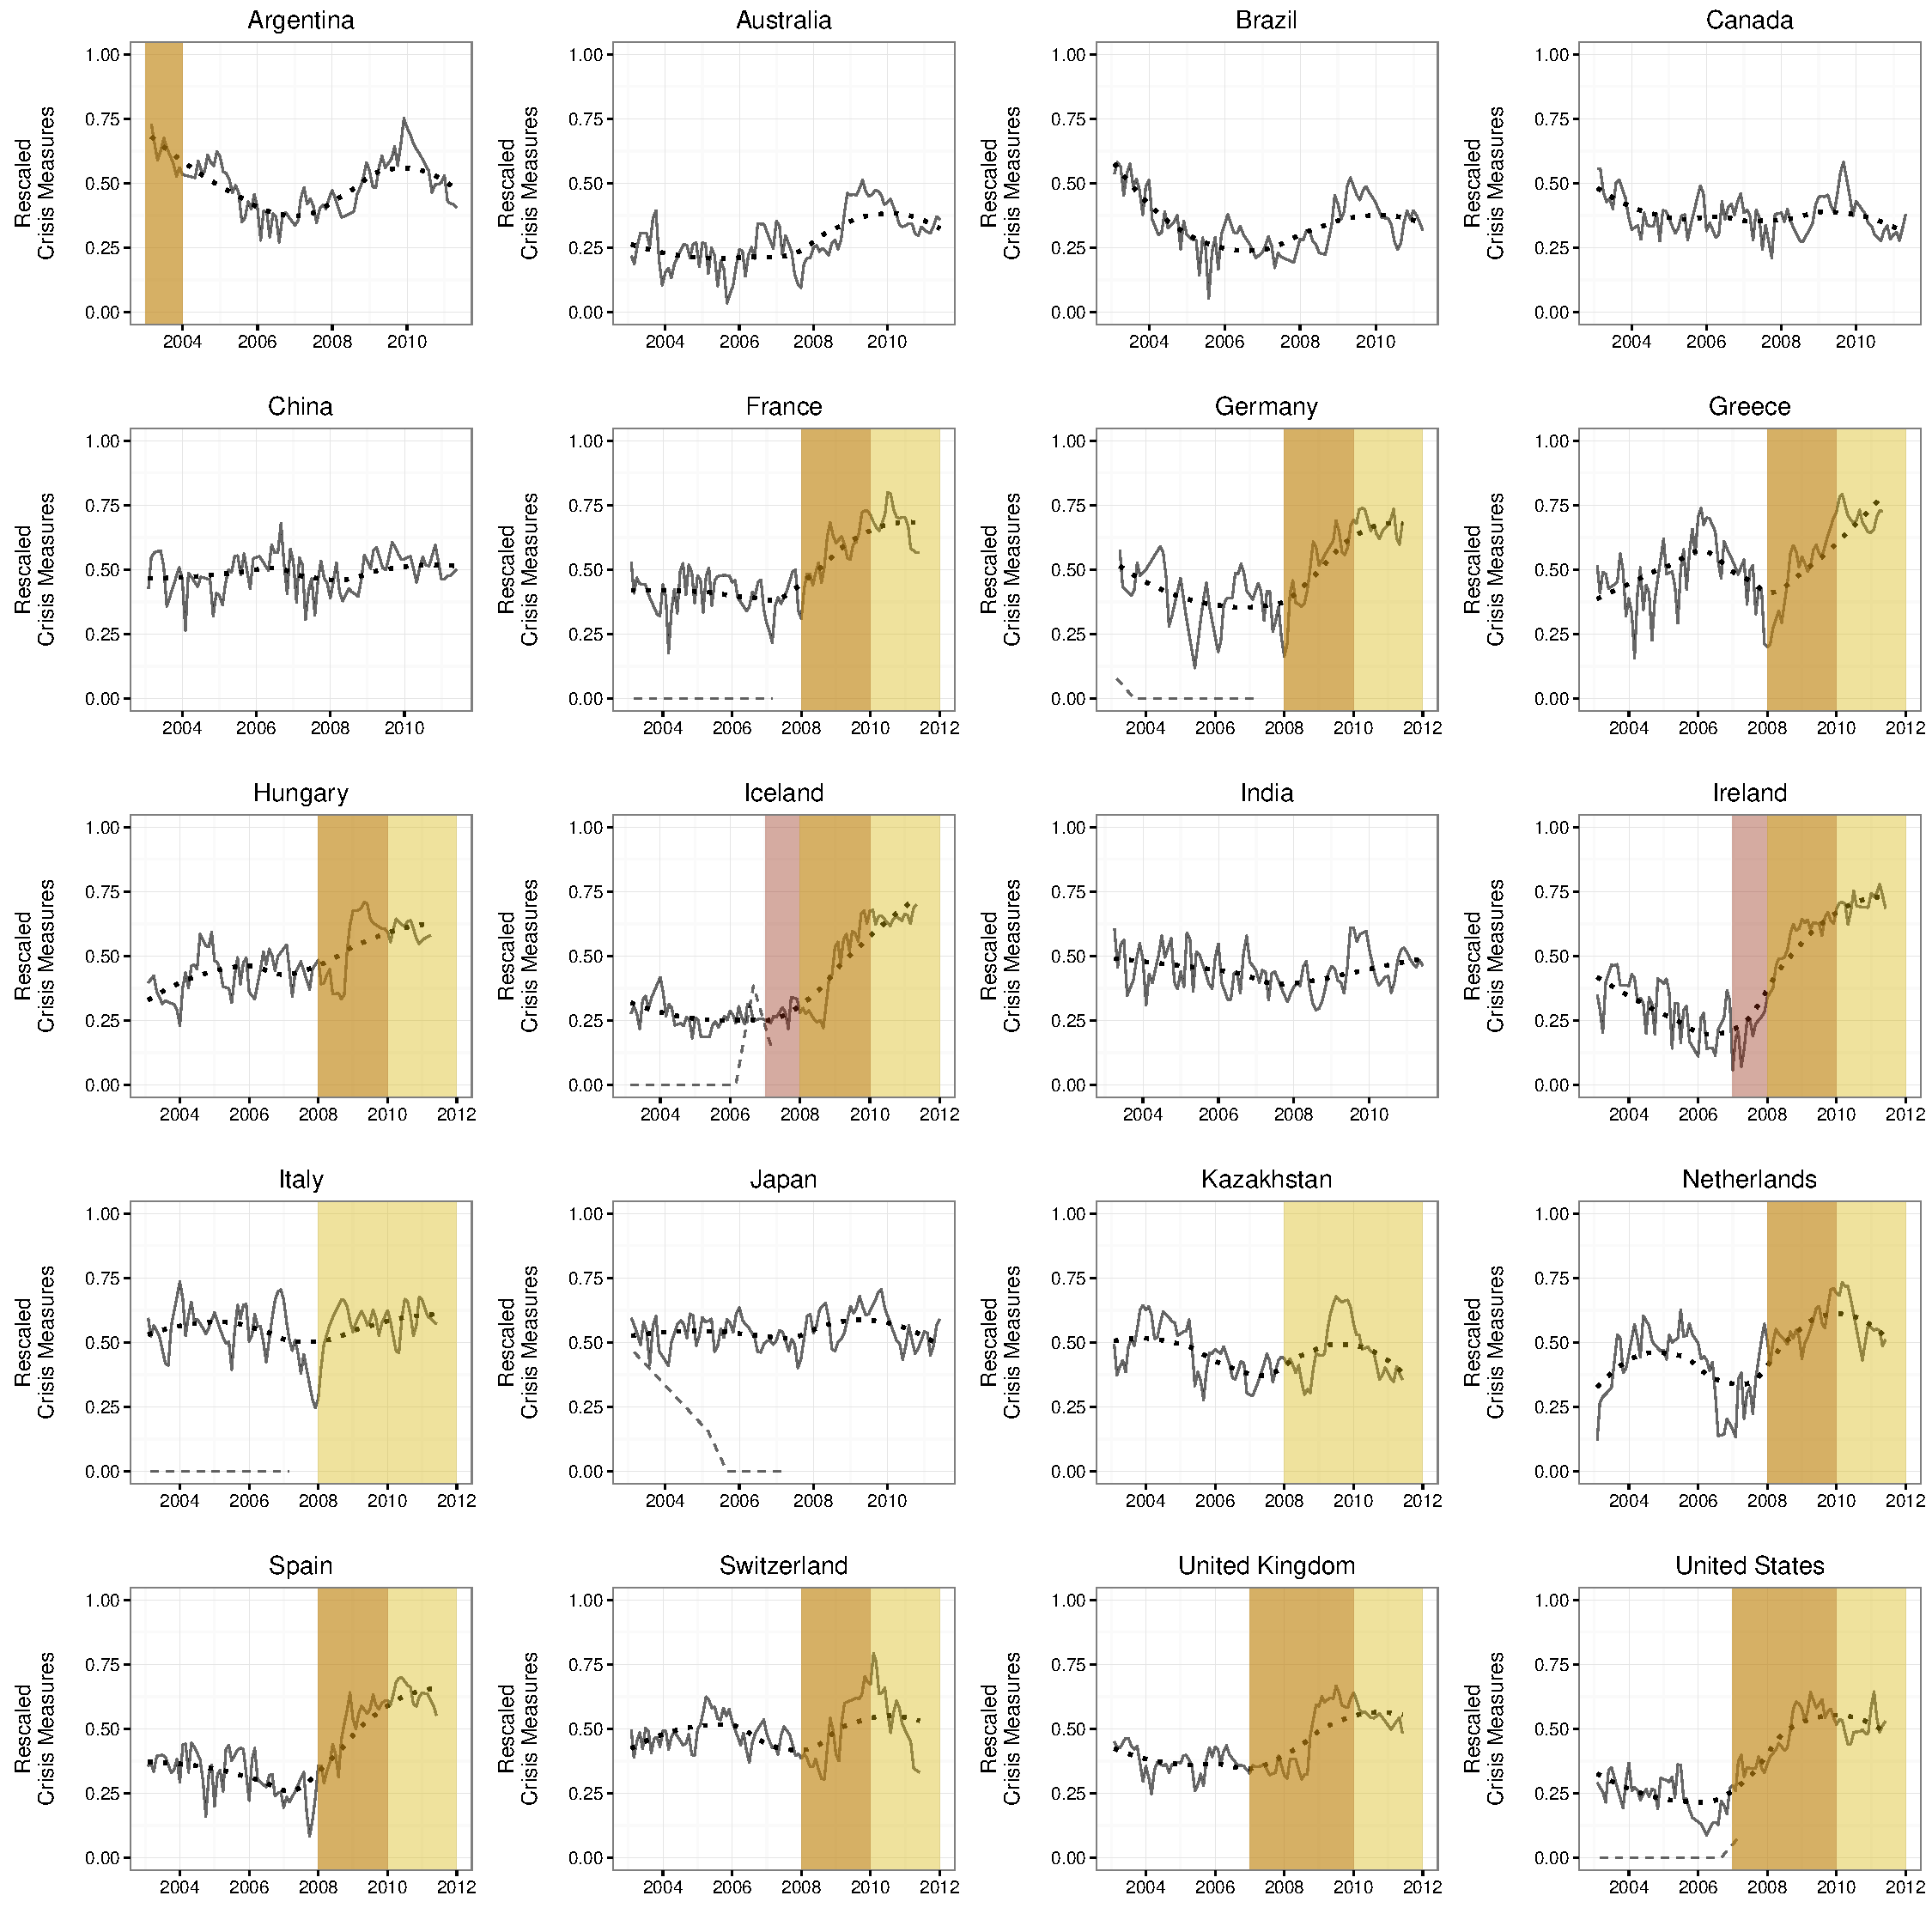
\includegraphics[scale=0.4]{figures/compare_to_lv_rr_short.pdf}
    \end{center}

    {\tiny{Solid lines show the FinStress Index. Dotted lines represent a loess smoother of these series. Dashed lines show the (rescaled) scores from \cite{Romer2015}. \\

    Yellow shaded areas indicate periods that \cite{laeven2013} classify as systemic banking crises. Crises are automatically terminated at the end of 2011 as the series does not extend beyond this point. \\

    Red shaded areas indicate periods that \cite{Reinhart2009} classify as banking crises. Crises are automatically terminated at the end of 2009 due to the series not extending beyond this point. \\

    Orange areas indicate periods where a crisis is recorded for both measures.}}
\end{figure}

\subsection{Comparison with other indices}\label{comparison-to-other-crisis-measures}

We now compare FinStress to the dichotomous measures of banking crisis developed by \cite{Reinhart2009} and \cite{laeven2013},\footnote{\cite{laeven2013} identify eight ``borderline'' crises in this period, in that the countries almost meet their systemic banking crisis definition because they only used two rather than three policy responses. These are: France, Hungary, Italy, Portugal, Russia, Slovenia, Sweden, and Switzerland.} as well as Romer and Romer's \citeyearpar{Romer2015} continuous measure.\footnote{We use Table 1 in \cite{Romer2015} to recreate their data set. The Laeven and Valencia's data is from: \url{https://www.imf.org/external/pubs/cat/longres.aspx?sk=26015.0}. Reinhart and Rogoff's data was downloaded from: \url{http://www.carmenreinhart.com/data/browse-by-topic/topics/7/}. Accessed May 2015.} We expect that our measure is capturing many of the same events, but with more nuance in magnitude and over time.

Figure \ref{compare_1} compares FinStress to three other measure of financial stress. In many cases--conditional on the coverage of each data series\footnote{\cite{Romer2015} do not include the most recent crisis in their sample as they did not collect data past 2007. We rescale their 16-point scale to be between 0 and 1. It should be noted that \cite{Romer2015} only cover a selection of OECD countries. \cite{Reinhart2009} only cover 70 countries and their data has been updated least recently.}--the indices substantively overlap. Comparisons with \cite{Romer2015} are limited, but we can see that, where comparable data is available, there are cases where FinStress and their index are similar. For example, both indices increase in the US from early 2007. A notable difference is how Romer and Romer classify Japan as being without stress from mid-2005, while FinStress decreases, but to a high level compared to many other economically developed countries at that time. Both indices classify Iceland as being under stress in the late 2000s, the timing is different. Romer and Romer classify Iceland as in stress\footnote{They classify Iceland as having a ``minor crisis'' in the second half of 2006 and a ``credit  disruption'' in the first half of 2007.} in 2006-2007. This is earlier than not only a marked increase in the FinStress Index, but also Reinhart and Rogoff and Laeven and Valencia's timing.

High FinStress levels should appear where there is crisis in the dichotomous codes, but the reverse may not be true--the dichotomous indices may miss a building crisis as perceived at the time. Laeven and Valencia and Reinhart and Rogoff should have more Type II errors--there are signs of stress but they miss them. Laeven and Valencia's coding is stricter because countries both have to experience distress and have a particular policy response, so the associated FinStress levels should be higher.

We do find that the mean FinStress level during periods that Laeven and Valencia classify as crises--i.e., financial market stress reached the point where politicians responded using a pre-specified set of policies--is higher than non-crisis periods.\footnote{0.59 and 0.52, respectively. This is a statistically significant difference using one-sided and two-sided t-tests.} Though developing countries tend to have higher FinStress scores, countries defined by Laeven and Valencia as in crisis in both groups have FinStress scores around 0.59 on average. Those not in Laeven and Valencia crises have lower scores.\footnote{See the Online Appendix for a discussion of the distributions of FinStress scores in developed vs. developing economies.} The fact that mean FinStress is higher during periods that Laeven and Valencia classify as crises, but not dramatically, supports the proposition that they miss considerable periods of budding and high stress and perhaps suffer from more Type II errors.

Laeven and Valencia \citeyearpar[227]{laeven2013} comment that part of the problem with dating financial crises is that each one develops differently:

\begin{quote}
    Some crises evolve gradually, gaining speed as the ripple effects from a seemingly small shock propagate forward in time \ldots other episodes happen more abruptly and are often the result of sudden stops.
\end{quote}

\noindent FinStress' real-time continuous measurement and monthly periodicity allows us to distinguish these types. We can see in Figure \ref{compare_1} that financial market difficulties in the United States built over a long period, with a few spikes during notable banking difficulties, e.g. Bear Stearns' and Lehman Brothers' collapse. Conversely, countries such as Germany, Hungary, and Iceland have more sudden periods of perceived financial distress. The Greek case presents an interesting trajectory. There is a notable spike in Greek financial stress in 2008--when both \cite{Reinhart2009} and \cite{laeven2013} determine a crisis had started. This is then followed by a stable period, followed by a sudden uptick in 2010, which was when a possible government default severely threatened the banking system.

Kazakhstan is notable for another path: rapid stress onset and just as rapid dissipation. In late 2009 there was a prominent spike in perceptions of stress directly related to a credit crunch resulting from the Global Financial Crisis. According to an IMF assessment,\footnote{See: \url{http://www.imf.org/external/pubs/ft/survey/so/2010/car081710a.htm}. Accessed November 2015} a large and quick policy response--facilitated by the country's sizable National Oil Fund--within a few months returned stability to the country's banking system. Kazakstan's FinStress score returns to almost its previous trend level at that time. Annual binary measures of crises do not capture these changes.

We can use FinStress to identify periods where financial market conditions were perceived to be worsening, though for whatever reason these perceptions changed before other measures would record a financial crisis. Australia in late-2008/2009 is a notable example. It had a clear spike in perceptions of stress shortly after Lehman Brothers' collapse. Fairly quickly thereafter, its FinStress scores returned to previous levels. Laeven and Valencia and Reinhart and Rogoff do not distinguish these periods.

FinStress' advantages are also apparent for timing the end of heightened  distress. This is a difficult issue for the binary indicators. Crisis onset is well-defined by these measures, but they rarely have a clear or non-\emph{ad hoc} way of determining when a crisis ended. Though we are limited by the time period coverage of the EIU texts, it is clear that some countries, notably Switzerland, the United Kingdom, and the United States, were perceived to have had improved financial market conditions from about 2010. Other countries, particularly Eurozone countries in Western and Southern Europe plateaued at a high level through the end of 2011, a period that corresponds with the Eurozone crisis. Laeven and Valencia's measure uses an \emph{ad hoc} definition of crisis termination and so classifies these entire periods as crises with equal intensity.

\section{Application}

We now provide examples of how FinStress can be applied in political science research and demonstrate that it performs as well or better than previous binary measures.

\subsection{Exploring the functional form of the relationship between crisis and electoral volatility}

Following the Global Financial Crisis there has been considerable interest in how financial stress may hasten government failure \citep{CrespoTenorio2014}, how crises increase electoral support for extremist parties \citep{Funke2015}, and how negative economic events and crises increase electoral volatility, i.e. the degree to which voters switch support for a party from one election to another \citep{Mainwaring2016,Hernandez2015}. \cite{CrespoTenorio2014} and \cite{Funke2015} both rely on Laeven and Valencia's binary measure, while \cite{Hernandez2015} use an even simpler measurement of crisis: whether or not an election occurred after November 2008.

\begin{figure}
\caption{Hypothetical Scenarios of Error in the Measurement of Financial Market Stress at Elections Using an Annual Binary Measure vs. FinStress}
\label{election_timing_error}

\begin{subfigure}[b]{0.5\textwidth}
\centering
\caption{Time Order Measurement Error}

\resizebox{\linewidth}{!}{
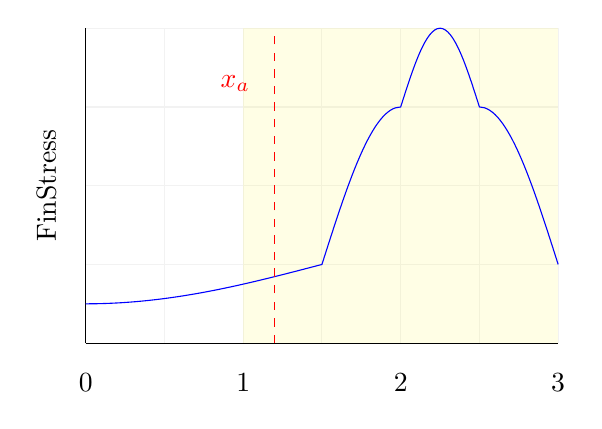
\begin{tikzpicture}

\node(t0) at (0,-0.5) {0};
\node(t1) at (2,-0.5) {1};
\node(t2) at (4,-0.5) {2};
\node(t3) at (6,-0.5) {3};

\node(yaxis)[rotate=90] at (-0.5, 2) {FinStress};

\draw[gray!10] (0,0) grid (6,4);

\draw[black] (0,0) -- (6,0);
\draw[black] (0,0) -- (0,4);

\fill[yellow, opacity=0.1] (2, 0) rectangle (6, 4);

\draw[blue] (0,0.5) cos (3, 1) sin (4,3) sin (4.5, 4) cos (5, 3) cos (6, 1);

\node(ax)[red] at (1.9, 3.3) {$x_{a}$};
\draw[red,dashed] (2.4, 0) -- (2.4, 4);

\end{tikzpicture}
}
\end{subfigure}
\begin{subfigure}[b]{0.5\textwidth}
\centering
\caption{Stress Intensity Measurement Error}

\resizebox{\linewidth}{!}{
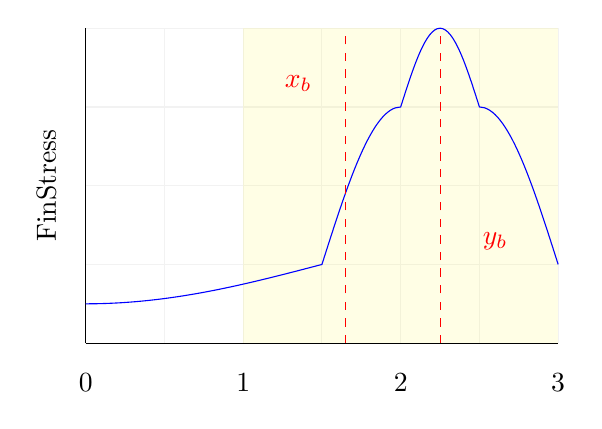
\begin{tikzpicture}

\node(t0) at (0,-0.5) {0};
\node(t1) at (2,-0.5) {1};
\node(t2) at (4,-0.5) {2};
\node(t3) at (6,-0.5) {3};

\node(yaxis)[rotate=90] at (-0.5, 2) {FinStress};

\draw[gray!10] (0,0) grid (6,4);

\draw[black] (0,0) -- (6,0);
\draw[black] (0,0) -- (0,4);

\fill[yellow, opacity=0.1] (2, 0) rectangle (6, 4);

\draw[blue] (0,0.5) cos (3, 1) sin (4,3) sin (4.5, 4) cos (5, 3) cos (6, 1);


\node(bx)[red] at (2.7, 3.3) {$x_{b}$};
\node(by)[red] at (5.2, 1.3) {$y_{b}$};

\draw[red,dashed] (3.3, 0) -- (3.3, 4);
\draw[red,dashed] (4.5, 0) -- (4.5, 4);

\end{tikzpicture}
}
\end{subfigure}

\begin{subfigure}[b]{0.5\textwidth}
\centering
\caption{Directional Change Measurement Issue}

\resizebox{\linewidth}{!}{
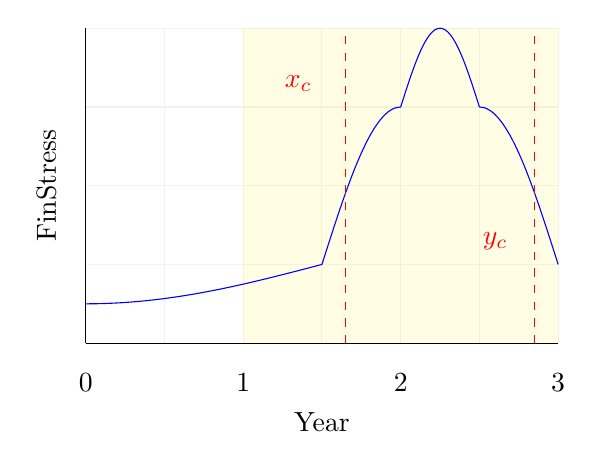
\begin{tikzpicture}

\node(t0) at (0,-0.5) {0};
\node(t1) at (2,-0.5) {1};
\node(t2) at (4,-0.5) {2};
\node(t3) at (6,-0.5) {3};

\node(xaxis) at (3, -1) {Year};
\node(yaxis)[rotate=90] at (-0.5, 2) {FinStress};

\draw[gray!10] (0,0) grid (6,4);

\draw[black] (0,0) -- (6,0);
\draw[black] (0,0) -- (0,4);

\fill[yellow, opacity=0.1] (2, 0) rectangle (6, 4);

\draw[blue] (0,0.5) cos (3, 1) sin (4,3) sin (4.5, 4) cos (5, 3) cos (6, 1);


\node(cx)[red] at (2.7, 3.3) {$x_{c}$};
\node(cy)[red] at (5.2, 1.3) {$y_{c}$};

\draw[red,dashed] (3.3, 0) -- (3.3, 4);
\draw[red,dashed] (5.7, 0) -- (5.7, 4);

\end{tikzpicture}
}
\end{subfigure}

{\scriptsize{
	Shaded area indicates years classified as a crisis by a binary crisis measure.
    Dashed vertical lines indicate an election.
}}

\end{figure}


Figure \ref{election_timing_error} presents hypothetical scenarios to illustrate measurement error when estimating the effect of financial market stress on elections. The top-left panel illustrates time-order measurement error. Using annual indicators of crisis may ascribe a level of stress to an election that was not perceived at the time. This type of error could lead to systematic under-estimation of the effect of financial market stress.

The upper-right panel of Figure \ref{election_timing_error} illustrates incorrectly measuring the intensity of financial market stress for two elections held during a period of heightened stress. Using a binary crisis measure codes the elections as occurring at equivalent stress levels. This error could lead to underestimation of the effect of crisis on election outcomes. Additionally, a binary measure would not allow us to examine if there was a non-linear effect of stress, e.g. perhaps very high stress has an exponentially stronger effect on outcomes than medium levels.

Finally, the lower-left panel of Figure \ref{election_timing_error} provides a scenario where both a binary crisis measure and FinStress levels would not capture potentially important features of how voters perceived stress at elections $x_{c}$ and $y_{c}$. Even though the binary and FinStress levels are the same in the former, stress is worsening, while in the latter conditions are improving. Voters might be more hostile to incumbents as conditions worsen and more favorable when conditions improve. The binary measure would not allow us to examine this possibility.

These are not just hypothetical examples. Figure \ref{elect_crisis_compare} compares national election dates in 19 European countries to FinStress scores and Laeven and Valencia crisis periods. There are elections where notably elevated FinStress levels and \cite{laeven2013} crises overlap. These include Belgium (June 2010), Germany (October 2009), and Iceland (May 2009). There are also notable examples of the binary crisis indicator coding an election as occurring in a crisis well before voters would likely have perceived one in their country. This includes Austria (October 2008), Portugal (October 2009), and Spain (March 2008). It would be inaccurate to estimate the effect of a crisis, which had not yet occurred, in these cases on voters' actions. There are also instances where financial market stress had declined or was notably declining by the time of the election, but the binary crisis measure still coded a full intensity crisis. This includes Sweden (October 2010) and the Netherlands (June 2010).

\begin{figure}
	\caption{Comparing National Election Timing, FinStress, and Laeven and Valencia's (2013) Banking Crisis Measure in Europe}
    \label{elect_crisis_compare}
    \begin{center}
		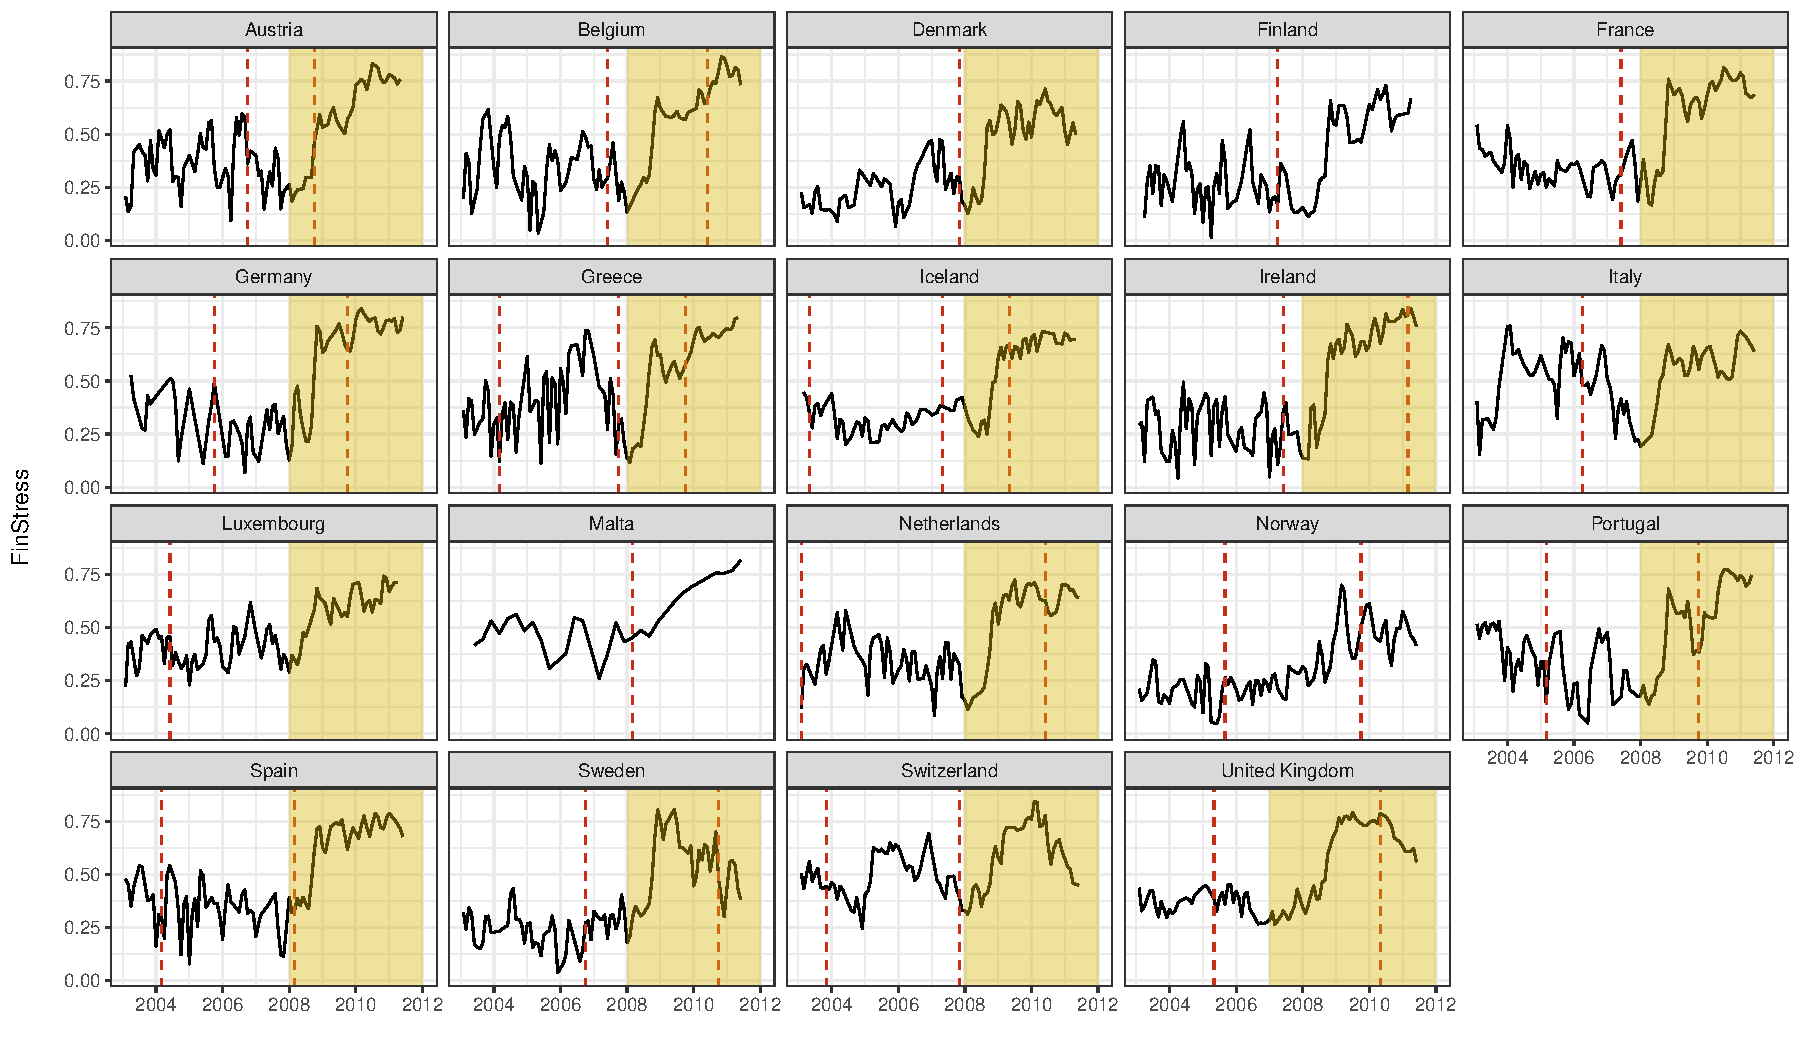
\includegraphics[scale=0.55]{figures/election_timing_crisis_comp.pdf}
	\end{center}
    {\scriptsize{Dashed vertical lines indicate national government elections.\\
    Yellow shaded areas represent \cite{laeven2013} banking crisis periods.
    }}
\end{figure}

In light of these measurement issues, and assuming that electoral volatility will be higher under more stressful economic conditions, we anticipate that the binary crisis measure will underestimate the effect of financial market stress on volatility compared to FinStress.

To examine this we use data on electoral volatility in Western European countries from \cite{Emanuele2015} which codes the total electoral volatility of an election by summing vote switching between existing parties, new parties, and failed parties. Because we aim to compare the estimated effects of the two financial market stress measures, we separately ran simple normal linear models of volatility including the stress measures on the right-hand side.\footnote{We are solely interested in comparing estimates between the stress measures and given our small sample size, other effects were consigned to the error term. The sample used is that shown in Figure \ref{elect_crisis_compare}.}

\begin{figure}
	\caption{Predicted Electoral Volatility for Representative Levels of FinStress and Laeven and Valencia (2013) Banking Crisis}
    \label{pred_vol}
    \begin{center}
		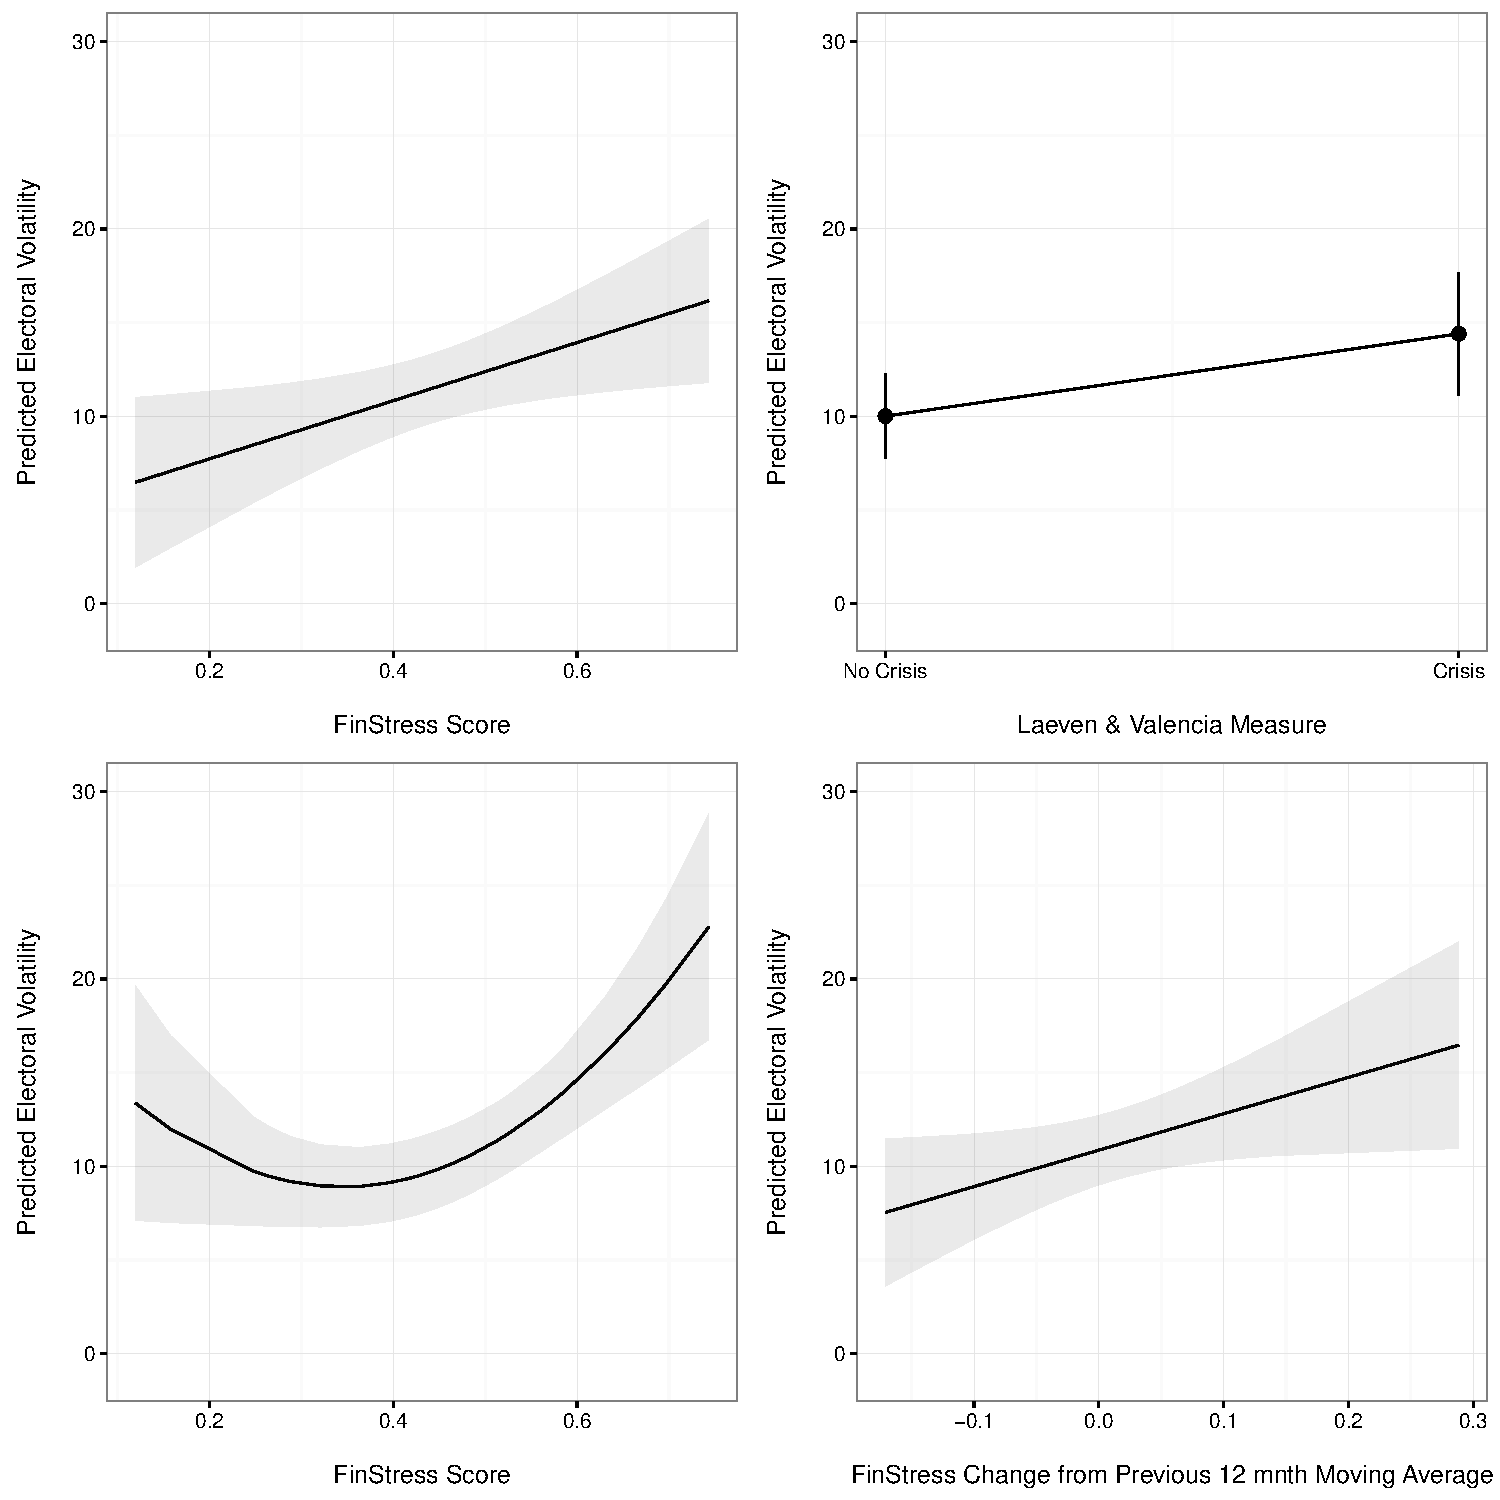
\includegraphics[scale=0.5]{figures/elect_vol_predict.pdf}
	\end{center}
    {\scriptsize{
    Shaded regions/vertical lines represent 95 percent confidence intervals.
    }}
\end{figure}

Figure \ref{pred_vol} shows predicted electoral volatility--which ranges from 2.5 to 29.6 in the sample--under various fitted levels and measures of stress. The first row of plots shows results from simple linear specifications. As expected, while both the binary and continuous measures are estimated to have a significant--at the 10 percent level--positive effect on volatility, the predicted effect of FinStress is somewhat stronger. The bottom-left panel of Figure \ref{pred_vol} shows predicted electoral volatility from a model estimated by adding a quadratic term. Above FinStress scores of about 0.6 we estimate a rapidly increasing effect of FinStress on volatility. At the highest levels, volatility is predicted to be much higher than anticipated by the binary measure of crisis and linear FinStress. The average predicted volatility at the highest FinStress levels under the quadratic specification is 20.9, while it is 15.3 in the linear FinStress specification and 14.4 for the binary measure.

The middle-left panel of Figure \ref{pred_vol} shows the predicted volatility for the range of observed changes to FinStress from the previous 12-month moving average. Large increases in stress compared to the average level over the previous 12 months is associated--at the 10 percent significance level--with increased electoral volatility. Stated conversely, improving financial market conditions are predicted to lead to less vote switching. The closest analogue to examining the effect of stress changes on volatility for the binary measure is to create a binary crisis-start year variable.\footnote{Following \cite{McGrath2015}, we drop observations for years after the start of a crisis. Given the arbitrary five year crisis termination coding used by \cite{laeven2013} and our limited sample, all crises were right-censored, we were not able to examine the effect of coming out of a crisis.} In contrast to the estimates with the FinStress change variable, we did not find a statistically significant effect at any level of Laeven and Valencia crisis onset on electoral volatility (Figure \ref{pred_vol}, middle-right panel).

\subsection{Comparing model fit}

We further compare the usefulness of FinStress to the Laeven and Valencia binary crisis measure by comparing the adjusted $R^2$ from models with the two indices. A higher adjusted $R^2$ would indicate that a variable explains more of the variance in the dependent variable.

We use regressions with electoral volatility as the dependent variable, as well as a substantively very different variable: cumulative revisions to EU member state government debt statistics made by the European Union's statistical agency--Eurostat. \cite{gandrudHallerbergJEPP} used this variable to examine the political and economic conditions associated with Eurostat--an independent statistical agency--revising government debt statistics. One of their findings was that governments facing unscheduled elections, during financial crisis were more likely to have their debt statistics revised upwards. The authors argue that this is likely because incumbents under-report debts during stressful times to make themselves more attractive to voters.

We ran identical linear regression models with the dependent variables, changing only whether we included FinStress, the FinStress polynomial discussed earlier, or the binary crisis measure. The results are shown in Table \ref{finlvregcompare} in the Online Appendix. For electoral volatility, the model with polynomial FinStress has an adjusted $R^2$ about 1.8 times higher than that with the binary measure (0.193 vs. 0.109). For debt revisions the difference is more modest, with the FinStress model having an adjusted $R^2$ 1.08 times that of the binary model (0.405 vs. 0.375). When using debt revisions as the dependent variable, monthly FinStress was collapsed into its annual average to put it on the same time scale as the annual dependent variable. It is not surprising that the relative model fit is better with monthly FinStress than when it is collapsed into an annual average, and thus more similar to the annual binary measure. The former is a context that leverages FinStress' continuous measurement level and high frequency, whereas the latter reduces this information.

\section{Conclusion}\label{conclusion}

We introduced a novel continuous measure of real-time perceived financial stress--FinStress--and compared it to prior measures of financial stress and crisis. We showed how this monthly continuous indicator--created with unsupervised text analysis--provides more accurate estimates of the impact stress has on political events like elections than less finely, but more laboriously constructed indicators.

Our methodological work has implications for the wider research community. We demonstrated how researchers could construct continuous indicators of other political and economic phenomena using machine learning and text analysis of large corpuses of similarly formatted texts. Once a text gathering and analysis ``pipeline'' \citep{Leek2015} has been developed and validated, researchers can efficiently estimate and update new indicators.\footnote{See the Online Appendix where we compare FinStress made with different sub-samples. These are very similar indicating that the method could be used to update an index when new documents become available within a consistently styled corpus.} This approach is especially useful in comparison to time-consuming, expensive, and irreproducible human coding techniques for collections of similarly formatted texts.

\bibliographystyle{apsr}
\bibliography{main.bib}

\pagebreak
\renewcommand{\thepage}{A-\arabic{page}}\setcounter{page}{1}
\renewcommand{\thesection}{Appendix \arabic{section}}\setcounter{section}{0}
\renewcommand{\thetable}{A-\arabic{table}}\setcounter{table}{0}
\renewcommand{\thefigure}{A-\arabic{figure}}\setcounter{figure}{0}
\clearpage

\section*{Online Appendix}

\begin{table}[H]
    \caption{Comparison of Binary Crisis Measures' Definitions}
    \label{comp_table}
    \begin{center}
        \begin{tabular}{m{3cm} | m{2cm} m{2cm} m{7cm}}
            Source & Measurement Level & Periodicity &  Definition of Financial Market Distress/Crisis \\
            \hline\hline
                Reinhart and Rogoff \citeyearpar[11]{Reinhart2009,ReinhartRog2010} & binary & annual & One of two types of events: (1) bank runs leading to closures, mergers, or public sector takeovers of one or more financial institution or (2) the closure, merger, takeover, or large-scale government assistant--at least three measures--of an important financial institution marking the start of a string of similar events.  \\[1cm]
                Laeven and Valencia \citeyearpar[228]{laeven2013} & binary & annual & Meets two conditions: (1) significant sign of financial distress in the banking system and (2) significant banking policy intervention measures in response to significant losses in the banking system.  \\[1cm]
            \hline
        \end{tabular}
    \end{center}
\end{table}

Laeven and Valencia define ``significant intervention'' as at least three of the following six policies being used: deposit freezes/banking holidays, significant bank nationalizations, bank restructuring gross costs, extensive liquidity support, significant guarantees, and significant asset purchases \citeyearpar[][229]{laeven2013}.

\subsection*{Selection of Literature Including Binary Cross-Country Measures of Financial or Banking Market Crisis}

\begin{table}[H]
\caption{Selected Literature Review of Political Institutions and Financial
Crisis (Binary Crisis Occurrence, Political Outcomes)}


\label{LitRevTable2}
\begin{center}

\vspace{0.5cm}
{\tiny{
\begin{tabular}{ m{2.5cm} m{1.75cm} m{6.25cm} m{2.5cm} }
    \hline
    Work & Crisis Type & Key Arguments/Findings & Crisis Data Sources \\
    \hline\hline

    %%% Bernhard and Leblang
    \cite{Bernhard2008} & Currency crisis & - Changes in the probability that cabinets will collapse condition the probability of speculative attacks.

    - Higher probability of a speculative attack decreases the probability of calling strategic elections. & Own data aggregated from multiple sources \\[0.25cm]\hline

    %%% Chwieroth and Walter
    \cite{Chwieroth2013} & Banking crises &  - Probability of government survival during crises changed over time as expectations changed about what governments should do to respond.

    - Governments with more veto players after the inter-war period are treated more harshly by voters. & \cite{ReinhartRog2010} \\[0.25cm]\hline

    \cite{CrespoTenorio2014} & Banking crisis & - Increasing globalization weakens the accountability link between politicians and voters.

    - Incumbents in open capital economies are more likely to survive a crisis, than those in closed economies. & Own data aggregated from multiple sources. \\[0.25cm]\hline

    %%% Montinola
    \cite{Montinola2003} & Banking crisis & - IMF credits decrease the probability of resolving banking crises.

    - The decisiveness of a political regime significantly influences the probability of emerging from systemic distress, though this depends on whether the crisis is moderate or severe. & Own data aggregated from multiple sources \\[0.25cm]\hline

    %%% Pepinsky
    \cite{Pepinsky2012} & Banking crisis & - Two factors--incumbent governments' responsibility for the current crisis and their responsiveness to its domestic economic effects--shape the political effects of the global economic crisis. & \cite{Laeven2010} \\[0.25cm]\hline

    \hline
\end{tabular}

}}
\end{center}
\end{table}

\begin{table}[H]
\caption{Selected Literature Review of Political Institutions and Financial
Crisis (Binary Crisis Occurrence, Policy Choices/Policy Outcomes)}


\label{LitRevTable}
\begin{center}

\vspace{0.5cm}
{\tiny{
\begin{tabular}{ m{2.5cm} m{2cm} m{7cm} m{3cm}}
    \hline
    Work & Crisis Type & Key Arguments/Findings & Crisis Data Sources \\
    \hline\hline

    %%% Broz
    \cite{broz2013} & Banking crisis & - In OECD countries right-wing governments pursue policies that lead to financial instability. Voters respond to resulting crises by voting in left-wing governments. & \cite{Reinhart2009,Laeven2012} \\[0.25cm]\hline

    %%% Galasso
    \cite{galasso2014} & Financial and economic crises & - Governments respond to financial crises by increasing regulation. & Dummy based on OECD output gap below -3.4\% \\[0.25cm]\hline

    %%% Gandrud
    \cite{Gandrud2013,Gandrud2014} & Banking crises & - Best practice financial governance institutional designs are more likely to be adopted during crises when there is high uncertainty about policy choices and outcomes. & \cite{Laeven2008,ReinhartRog2010} \\[0.25cm]\hline

    %%% Ha and Kang
    \cite{ha2015} & - Banking crisis & Developing countries respond to crises with fiscal and monetary tightening, which was moderated by political constraints, left ideology governing parties, and up coming elections. & \cite{Laeven2008}. \\[0.25cm]\hline

    %%% Hallerberg Scart
    \cite{HallerbergScartForthcoming} & Banking, debt crises & - Banking crises reduce the probability of fiscal reforms, but the longer a crisis lasts and if it becomes a sovereign debt crisis the the probability of reform increases.

    - Countries with more personalistic voting are more likely to reform. & \cite{Laeven2012} for Latin American countries \\[0.25cm]\hline

    %%% Hallerberg Wehner
    \cite{Hallerberg2013} & Banking, currency, debt crises & - Some evidence that more technically competent ministers of finance are appointed during debt crises. Not much robust evidence for other effects of crisis on the technical competency of economic policy-makers. & \cite{Laeven2012}  \\[0.25cm]\hline

    %%% Hicken et al.
    \cite{Hicken2005} (2005) & Growth shocks & - The size of the winning coalition is positively associated with growth recoveries following forced devaluations. & Own data aggregated from multiple sources \\[0.25cm]\hline

    %%%% Keefer
    \cite{Keefer2007} & Banking crises & - Higher electoral competitiveness leads to faster and less costly crisis responses.

    - Checks and balances not associated with crisis policy choices or outcomes. & Modified \cite{Honohan2003} \\[0.25cm]\hline

    %%% Kleibl
    \cite{Kleibl2013} & Banking crisis & - Responses to regulatory failures are conditioned by the level of public ownership in the banking sector. & \cite{Laeven2010,Reinhart2009} for OECD countries \\[0.25cm]\hline

    %%% MacIntyre
    \cite{MacIntyre2001} & Financial crises & - U-shaped relationship between veto players and crisis outcomes & Own data aggregated from multiple sources \\[0.25cm]\hline

    %%% Reischmann
    \cite{reischmann2015} & Banking crises & - Creative accounting as measured by changes in the stock flow adjustment occurs more during financial crises, though effect may be swallowed up by the period fixed effects in his regressions as crises are highly correlated with time in his sample. & \cite{Laeven2012} \\[0.25cm]\hline

    %%% Rodrick
    \cite{Rodrick1999} & Growth shock & - Many veto players, if organized to manage conflicts, will result in more appropriate and quickly implemented crisis management policies. & Own data aggregated from multiple sources \\[0.25cm]\hline

    %%%% Rosas
    \cite{Rosas2006,Rosas2009} & Banking crisis & - Democratic regimes have fewer bailouts.

    - Central bank independence and transparency lead to fewer bailouts. & Modified \cite{Honohan2000} \\[0.25cm]\hline

    %%% Seiferling and Tareq
    \cite{seiferling2015} & Banking crisis & - Find advanced economies governments extend more loans and purchase more equities in temporarily insolvent firms during financial crisis than emerging market governments. & \cite{Laeven2010} via \cite{weber2012} \\[0.25cm]\hline

    %%% Satyanath
    \cite{Satayanath2006} & Banking crises & - Executives without `banking cronies' and that are not prevented from appointing their own bureaucrats by many veto players are more likely to have stringent financial regulation that prevents crises. & Case studies of 7 East Asian countries using own data \\[0.25cm]\hline

    %%% Wibbels and Roberts
    \cite{Wibbels2010} & Currency, growth, \& fiscal crises & - Unions and strong left parties are more associated with crises, though combined strong unions-left parties may alleviate inflationary crises. & Own data aggregated from multiple sources for 17 Latin American countries \\[0.25cm]\hline


    \hline
\end{tabular}

}}
\end{center}
\end{table}

\subsection*{Further discussion of continuous financial market stress measures}

Another approach is to measure stress and crisis using nationally aggregated quantitative accounting data. The finance literature relies on a statistical quantity known as Z-Scores. The concept was originally developed to assess firm solvency \citep[see][]{roy1952}. In the banking context, it is often used to measure national financial system fragility, which allows researchers to examine how banking system structures and policies affect the probability of financial system difficulties \citep[e.g.][]{beck2013bank,vcihak2010islamic,laeven2009bank,uhde2009}. Though there are various ways to calculate this measure \citep[73]{Lepetit2013}, bank accounting information--assets, equity, and return on assets--is typically used to create an inverse measure of the probability that a country's banking system will become ``insolvent''.

Similarly, the CAMELS system uses accounting data to rate bank soundness. The CAMELS indicators include a bank's capital adequacy, asset quality, management capacity, earnings, the liquidity of its assets, and its sensitivity to market risks. \cite{Andrianova2015} gathered individual bank data from the Bankscope service on these quantities for 128 countries, created annual national aggregates, and released the components in a ``database on financial fragility''.

Research looking at longer time spans has been limited by what data is available at the bank-level for measuring banking system health. \cite{Danielsson2015} examine the Minskian \citeyearpar{Minsky1982} hypothesis that stable conditions in the present induce increased risk-taking behavior and thus crises in the future with annual stock market volatility. This data allows them to cover a period of 211 years. It seems plausible that stock market volatility is positively associated with broader financial market volatility. Nonetheless, it is well understood in political economy \citep[seminally][]{hall2001introduction} that the importance of equity markets for financing banks and the ``real'' economy varies considerably by country and over time.

There have been a number of further innovations to the measurement of banking system stability using quantitative data. Though they make interesting contributions to measuring financial market stress, these indicators have not been used in applied research as frequently as Z-Scores or CAMELS components. Building on \cite{vonHagen2007}, \cite{Jing2015} develop an index of money market pressure based on changes in short-term interest rates and stocks of central bank reserves. Problematically for the study of policy responses, it assumes that central banks use the same reaction function to increased demand for liquidity. \cite{Rosas2009dltm} developed a dynamic latent trait model of banking system distress. His measure relies on nationally reported data to the IMF's International Financial Statistics (IFS).

Most simply, we could perhaps use individual indicators from the IFS or the broader Global Financial Development Database \citep[GFDD,][]{worldbank2015}, such as the provision of private sector credit by deposit banks as an indicator of credit conditions or non-performing loan ratios as an indicator of bank balance sheet health. However, there are a number of issues.

First, as mentioned before, the importance of each individual measure varies depending on the context. Second, how these indicators are measured can vary significantly across countries. Many of the GFDD indicators have a note attached that ``due to differences in national accounting, taxation, and supervisory regimes, these data are not strictly comparable across countries''. Third, \cite{cghBruegel2015} show that national reporting to the IFS and GFDD is highly uneven across countries and time. As such, they indicate that decisions to report data could be endogenous to economic and political events, complicating attempts to use these data. They find that reporting on credit market conditions declined significantly in the European Union in the lead up to and during the crisis beginning in 2007. Further indicating the pervasiveness of the missingness problem with quantitative data, \cite{Andrianova2015} extensively discuss problems of missingness in their privately gathered database on financial fragility and caution users of the database about the effects it might have on their analysis. Fourth, as \cite{KayserLeininger2015} show, people make decisions based on contemporaneously available information, but researchers attempting to understand this behavior use data that has been significantly updated after the fact. Similar to the binary crisis indicators' \textit{post hoc} measurement problem, using revised IFS and GFDD data gives an inaccurate impression of the conditions that politicians believed they faced at the time.

\subsection*{KPCA comparison with \cite{Minhas2015}}

Our approach is broadly similar to \cite{Minhas2015} who use a supervised machine learning approach called support vector machines and United States State Department Country Reports on Human Rights Practices to classify countries according to dichotomous regime types. Our work is distinct in that KPCA of EIU reports allows us to develop a continuous measure of perceived financial market stress. Perhaps more importantly, their supervised learning approach assumes that countries have been well classified by previous indicators, which they use to train their model. As discussed above, we are not confident that previous measures do well classify high and low stress periods. Therefore, we use the unsupervised KPCA approach to establish new estimates.

\subsection*{Text selection and pre-processing}\label{text-selection}

EIU reports assess many economic sectors within a country,
not just the financial sector.
Our first step was to select the portions of the EIU texts that contained relevant information about countries' financial systems. We automatically collected and parsed the reports from their original HTML format. We then extracted the portions of the texts--headers and paragraphs--that contained at least one of a number of keywords concerning financial markets.\footnote{The
  keywords included: \emph{bail-out}, \emph{bailout}, \emph{balance
  sheet}, \emph{balance-sheet}, \emph{bank}, \emph{banks},
  \emph{banking}, \emph{credit}, \emph{crunch}, \emph{default},
  \emph{finance}, \emph{financial}, \emph{lend}, \emph{loan},
  \emph{squeeze}. These keywords are adapted
  from those used by \cite{Romer2015} and are intended to
  select passages that discuss credit market conditions. Note that a small number of the words, primarily \emph{bank} and \emph{financial} are by far the most selective.} Due to a significant change in the reports formatted in 2003, we selected only texts from 2003 in order to maintain comparability across the time-series. The texts from 2003 follow the same format and style and contain directly comparable assessments of economic conditions across the globe over a significant time span.

We also pre-processed the selected texts using standard techniques \citep[see][]{Grimmer2013}. This involved removing common English words, such as `was' and `its'. The `stopword' list we used to do this was from \cite{dhillon:modha:mlj01}. We stemmed the words so that different variants of the same word are represented by a common `stem'. This allowed us to work with a more manageable number of kernels. We removed extra white space between the words, as well as punctuation--with the exception of apostrophes indicating possession--and numbers. Finally, we dropped texts that included very few words (less than six). In practice, including these texts hindered the estimation of the KPCA model. All pre-processing was done using the \texttt{quanteda} package \citep{quantedaCite} in R \citep{R-cite}.

\subsection*{Dimensionality}\label{dimensionality}

To determine the number of dimensions from the KPCA that best describe the data, we conducted a scree test, with results in Figure \ref{scree_plot}. There is a clear ``elbow'' in the plot at component two. This suggests that the first component explains the most variation in the data. As such, FinStress is created from the first dimension as it is the main dimension summarizing financial market stress. We examined a number of the other dimensions. However, these did not correspond to our priors about financial market stress based on previous indicators. For example, Figure \ref{c1c2} compares FinStress to the second component, which has been transformed using the same procedures. It is difficult to discern consistent substantive meaning--at least for financial market stress--from the second component. Strikingly for Spain and the United Kingdom it does not reflect widely reported financial market stress in these countries in the latter part of the sample.

Given that components other than the first component do not appear to be substantively meaningful, we focus on the most parsimonious output of the KPCA analysis--the first component.

\begin{figure}
    \caption{Assessing Model Fit: Eigenvalues for Kernel Principal Components}
    \label{scree_plot}
    \begin{center}
        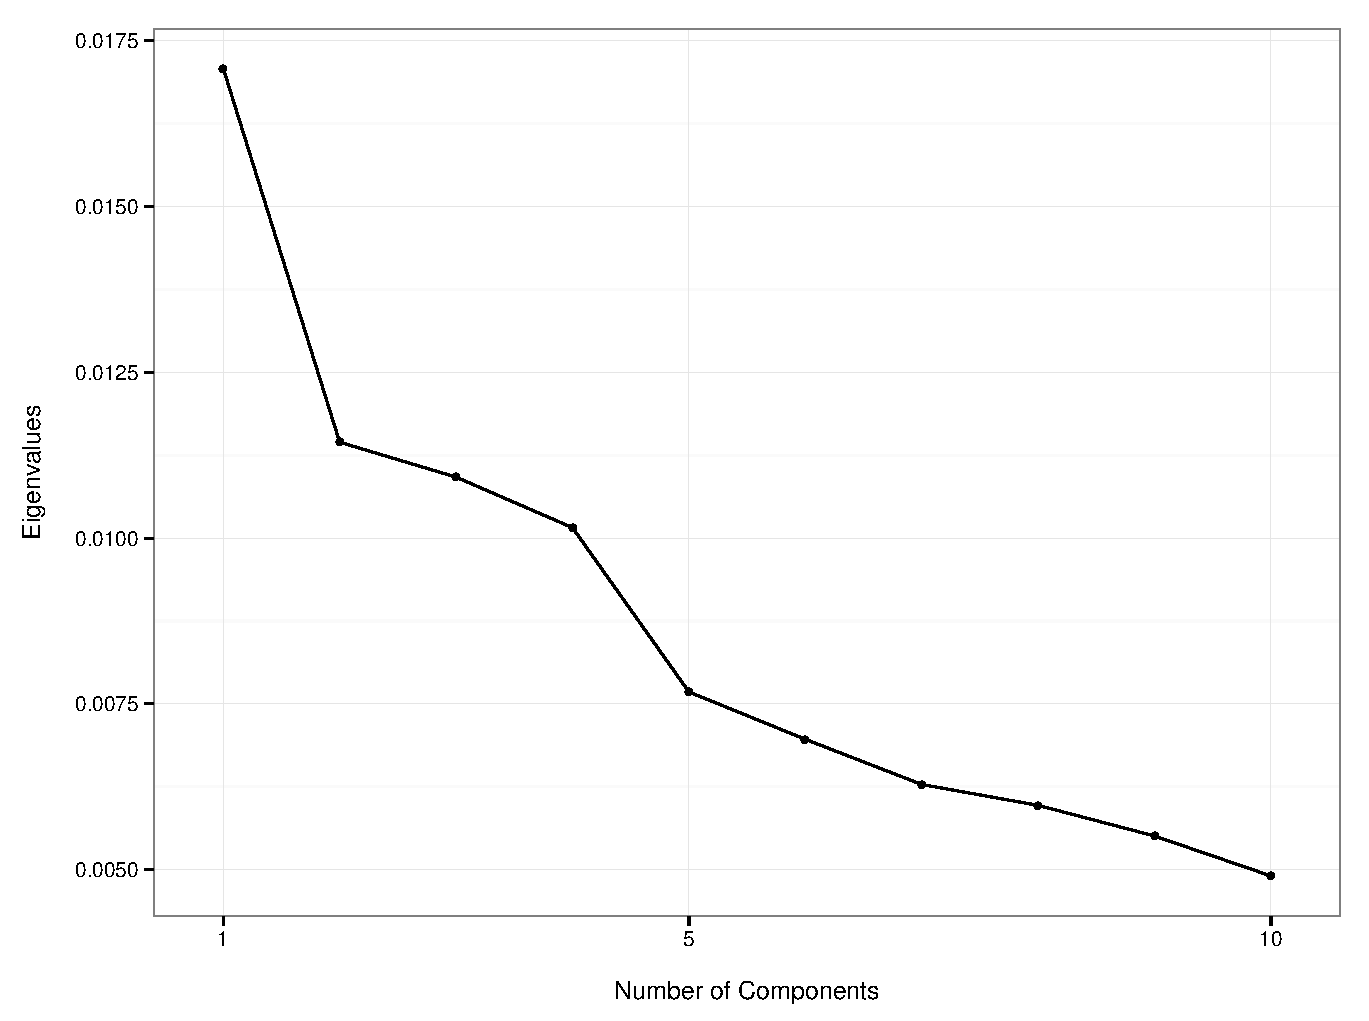
\includegraphics[scale=0.45]{figures/scree_plot.pdf}
    \end{center}
\end{figure}

\begin{figure}
	\caption{KPCA First Component (FinStress) vs KPCA Second Component (select countries)}
	\label{c1c2}
    \begin{center}
    	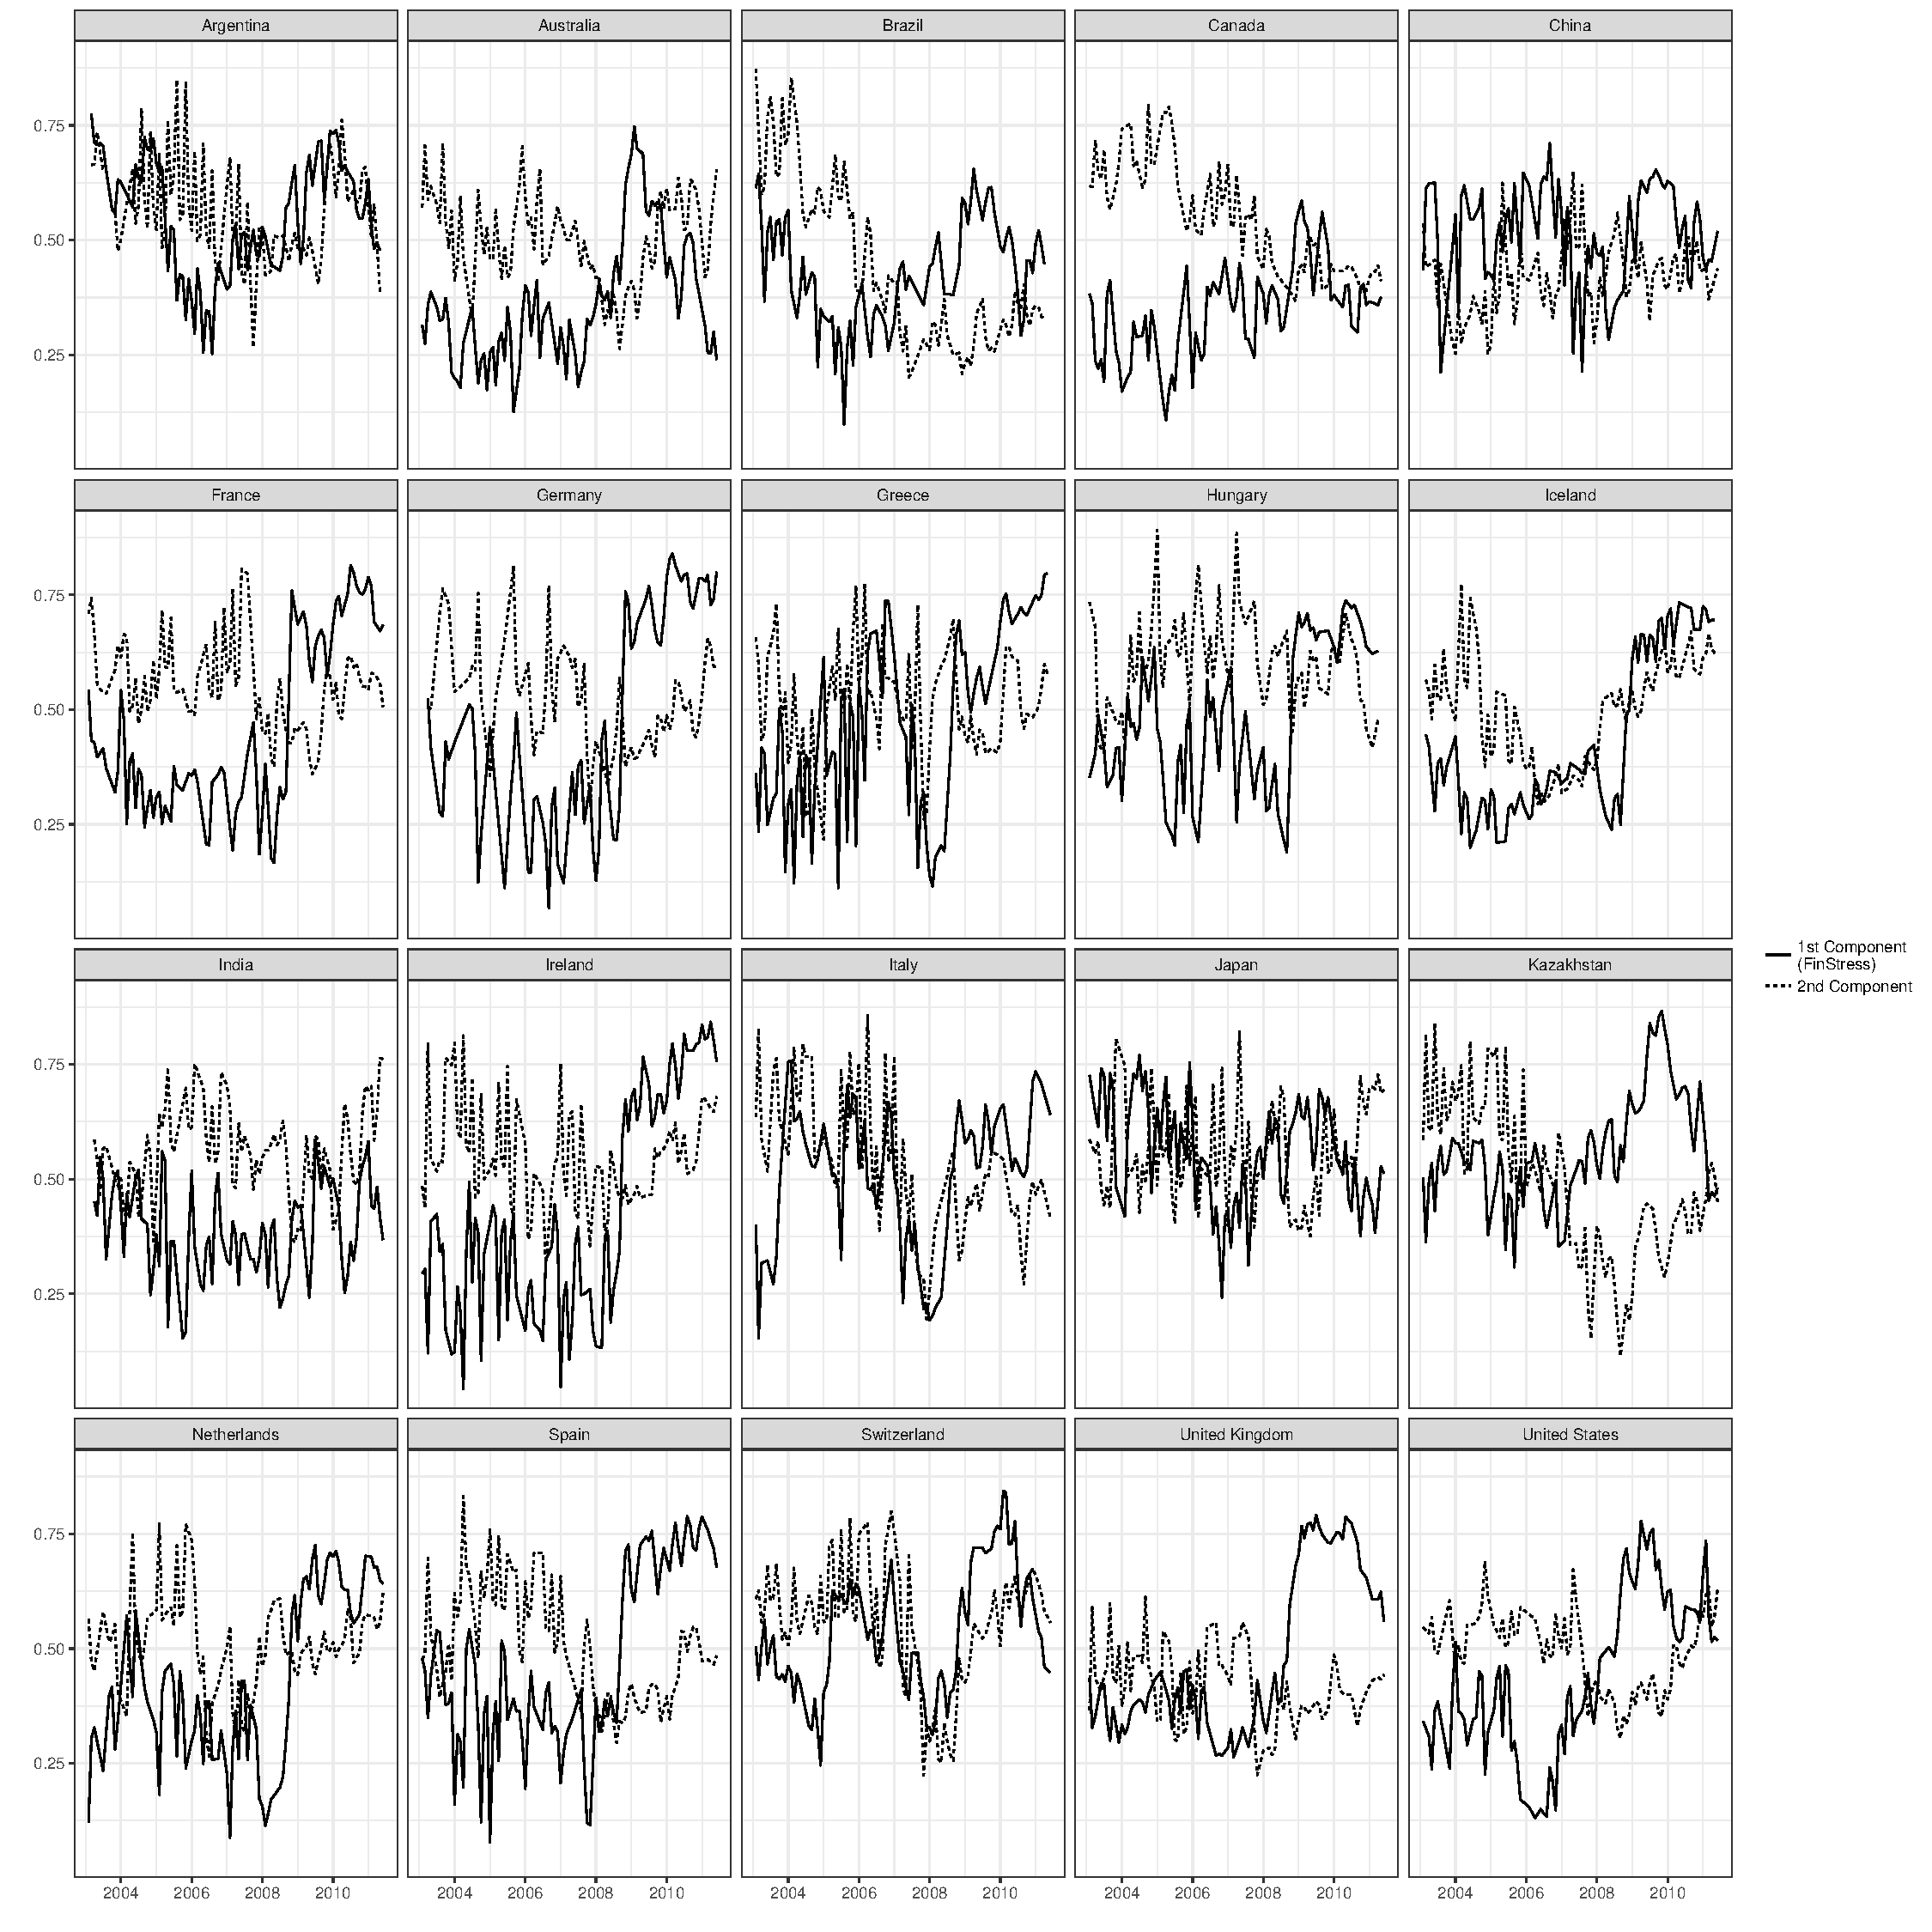
\includegraphics[scale=0.45]{figures/1st_vs_2nd_component_selected.pdf}
    \end{center}
    {\scriptsize{Both components were transformed using the same procedures discussed in the text.}}

\end{figure}

\subsection*{FinStress validity: random forests}\label{random-forests}

Spirling \citeyearpar[88-90]{Spirling2012} demonstrated the usefulness of using random forests regressions \citep{Breiman2001,jones2015} to explore what principal components from textual analyses represent. To do this, we first created a document-term frequency matrix from the stemmed documents. Effectively this is a \(k \times s\) matrix recording the frequency of each stem in \(\bm{S}\) for each document in \(\bm{K}\). \emph{The document-term matrix clearly does not preserve word order, so should only be thought of as a partial method of assessing validity}. We removed sparse terms, i.e.~kept only stems that were found in 90 percent of the documents. Random forests regressions, as opposed to ordinary least squares regressions, are useful for exploring this data's associations with the estimated principal components because it can handle many variables--in this case 921 stems--relative to the number of documents--12,373.

We focus on estimated variable importance. Variable importance in this context functions as a measure of how well the frequency of a given stem in a text allows the model to predict the FinStress score for that text.\footnote{Specifically, importance is measured in terms of the percentage increase in mean squared error (MSE) after permuting the variable. If a variable is important, then permuting it will decrease predictive performance, i.e. increase MSE. We conducted the random forests regressions using the \texttt{rfsrc} function from the \textbf{randomForestSRC} R package \citep{randomForestSRCCite}.} Key results are shown in Figure \ref{rf_importance}.

Unsurprisingly, a number of the stems with the largest variable importance are ``bank'', ``financi'', and ``loan''. Terms with these stems were used to select the texts. The prevalence of these terms and others that are clearly related to the financial sector, such as ``interest'', ``rate'', and ``fund'', indicate that FinStress is indeed about financial sector conditions and not some other topic. Words relating to the direction of financial conditions are important including, ``growth'' and ``tighten''. Words relating to the macro-political economic environment of finance are also important, including ``govern'' and ``imf''.

\begin{figure}
    \caption{40 Stems Estimated to be the Most Important for Predicting EIU Perception of Financial Market Stress Index}
    \label{rf_importance}

    \begin{center}
        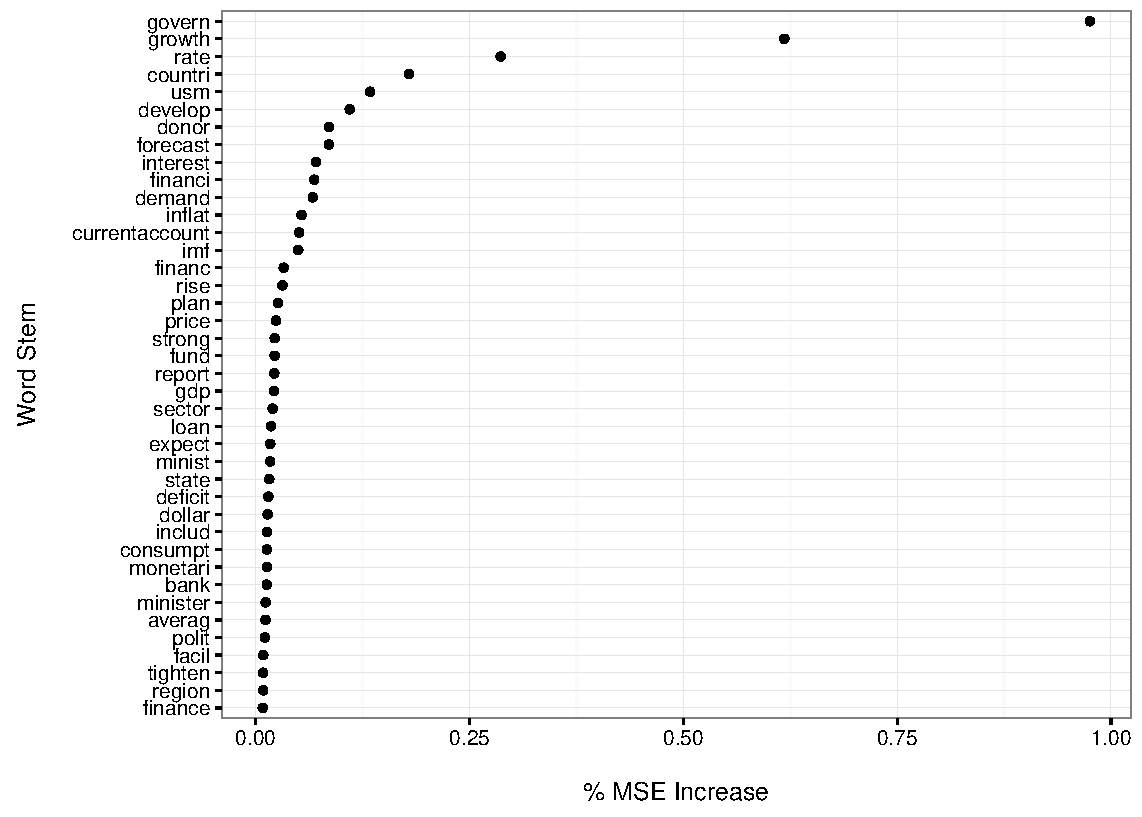
\includegraphics[scale=0.5]{figures/rf_stem_importance.pdf}
    \end{center}

\end{figure}

\subsection*{FinStress validity: word-stem component correlations}

Table \ref{stem_correlations} shows a selection of correlations to provide a sense of the general directions of the relationships between the stems and the Index not provided by the random forest variable importance estimates. A number of terms related to debt, financial assistance, the International Monetary Fund (IMF), and aid are positively related to FinStress. This suggests that the positive direction of the scale is in fact capturing periods where policymakers perceive higher financial market stress. Words that are generally about positive credit conditions, such as ``growth'', ``surplus'', and ``boom'' are negatively associated with the Index. This suggests that the lower end of the scale indeed indicates more positive financial market conditions. Finally, we can see that adjectives that have seemingly opposite meanings--``stronger'' and ``weaker''--are both negatively associated with the Index. Such findings indicate that a KPCA approach is useful compared to context-less bag-of-words sentiment analysis approaches based on individual word stems.

% latex table generated in R 3.2.1 by xtable 1.7-4 package
% Mon Jun 29 14:16:00 2015
\begin{table}[ht]
\centering
\caption{Selection of Word Stems and Correlations with EPFMS Index} 
\label{stem_correlations}
\begin{tabular}{lr}
  \hline
Stems & Correlations \\ 
  \hline
imf & 0.34 \\ 
  assist & 0.34 \\ 
  aid & 0.28 \\ 
  debt & 0.24 \\ 
  paid & 0.19 \\ 
  strain & 0.09 \\ 
  boom & -0.14 \\ 
  surplus & -0.14 \\ 
  rise & -0.14 \\ 
  weaker & -0.16 \\ 
  stronger & -0.17 \\ 
  growth & -0.28 \\ 
   \hline
\end{tabular}
\end{table}



\subsection*{FinStress compared to a bag-of-words principal components analysis}

KPCA allows us to utilize word order information, which we argued in the main paper is particularly important for gaining an accurate understanding of the perceived stress levels communicated in the EIU corpus. However, KPCA achieves this at non-trivial computational expense.\footnote{The scores with 5-character kernels were estimated using KPCA a 2014 iMac with 16GB of RAM and a 2.93 GHz Intel Core i7 processor. On this system the analysis took 3.68 days (318,316.2 seconds).} Perhaps a simpler method that did not preserve word order would be less computationally expensive with little loss in validity? To test this we conducted a traditional ``bag-of-words'' principal components analysis (PCA) on the texts and compared the results to FinStress.

We started this analysis with the same preprocessed corpus as the KPCA we used to create FinStress. We converted this corpus into a document-term matrix that did not preserve term order within the documents. Due to the large number of unique words, even after stemming and other preprocessing was conducted on the EIU corpus for the KPCA analysis, we were unable to run PCA on this document-term matrix. The number of terms exceeded the number of documents and so violated a key constraint of PCA. As such we removed sparse terms from the corpus, keeping only those that were present in 90 percent of the texts. We then ran the PCA analysis and selected the first component, rescaled it using the same procedures as for the FinStress Index. Finally we smoothed it with a two-period moving average, again as we did with FinStress.

The computation time for the bag-of-words PCA was trivial--under eight seconds--and the resulting estimates are positively and statistically significantly correlated with FinStress at all standard significance levels. However, with a correlation coefficient of 0.22, the magnitude of the relationship is not large. To examine the relative validity of the two measures, we directly compared the two sets of estimates for a diverse set of countries. These are shown in figures \ref{pcaCompare1} and \ref{pcaCompare2}. While there are some similarities, overall the bag-of-words created PCA estimates miss significant known crisis points that are accurately captured by FinStress. For example, the Irish 2008 crisis is accurately captured as starting in late 2008--when the government instituted large bank guarantees in response to imminent bank collapses \citep{gandrud_okeeffe2016}--by a dramatic increase in FinStress in late 2008. Ireland's PCA results also increase dramatically, but not until much later in 2010. Increased financial market stress is completely missed by the bag-of-words PCA estimates for a number of countries including Austria, Belgium, Denmark, Greece, Hungary, Iceland, and Spain.

While estimating the bag-of-words PCA was computationally much less intensive than using KPCA, it produced much less valid results. As such, the added computational effort involved in using KPCA is an appropriate cost for creating a more valid index of perceptions of financial market stress.

\begin{figure}
	\caption{FinStress Estimates Compared to PCA Bag-of-words Estimates (1)}
    \label{pcaCompare1}
    \begin{center}
    	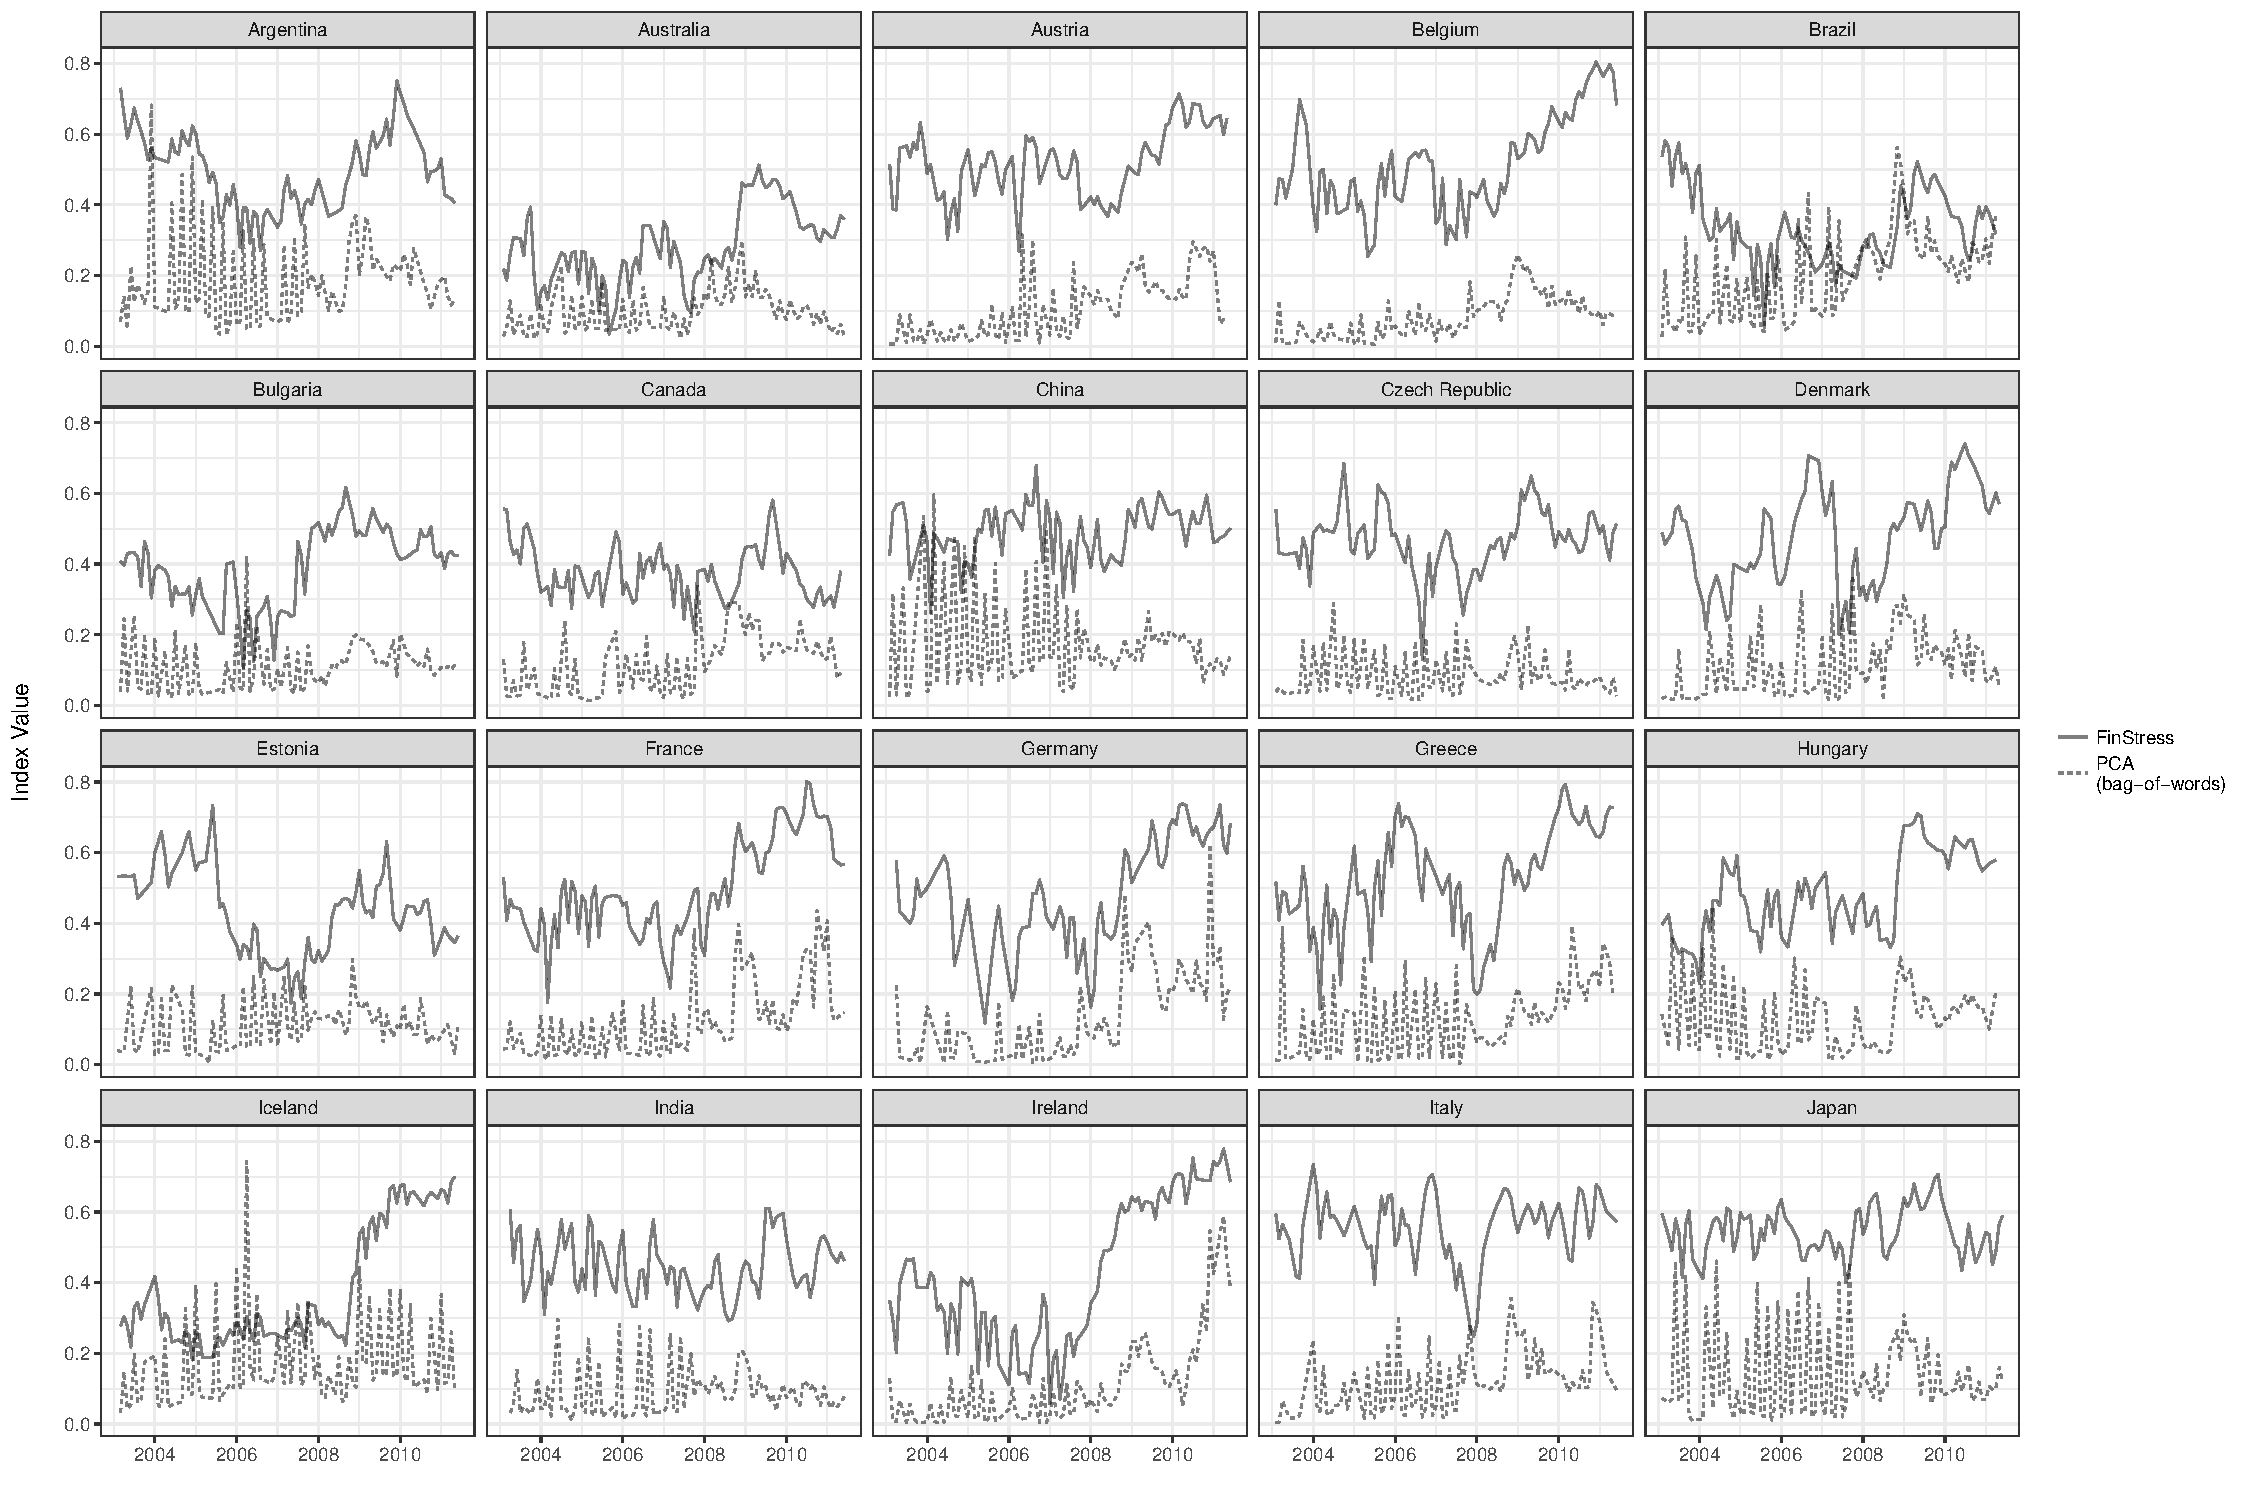
\includegraphics[scale=0.4]{figures/compare_to_pca_1.pdf}
    \end{center}
\end{figure}

\begin{figure}
	\caption{FinStress Estimates Compared to PCA Bag-of-words Estimates (2)}
    \label{pcaCompare2}
    \begin{center}
    	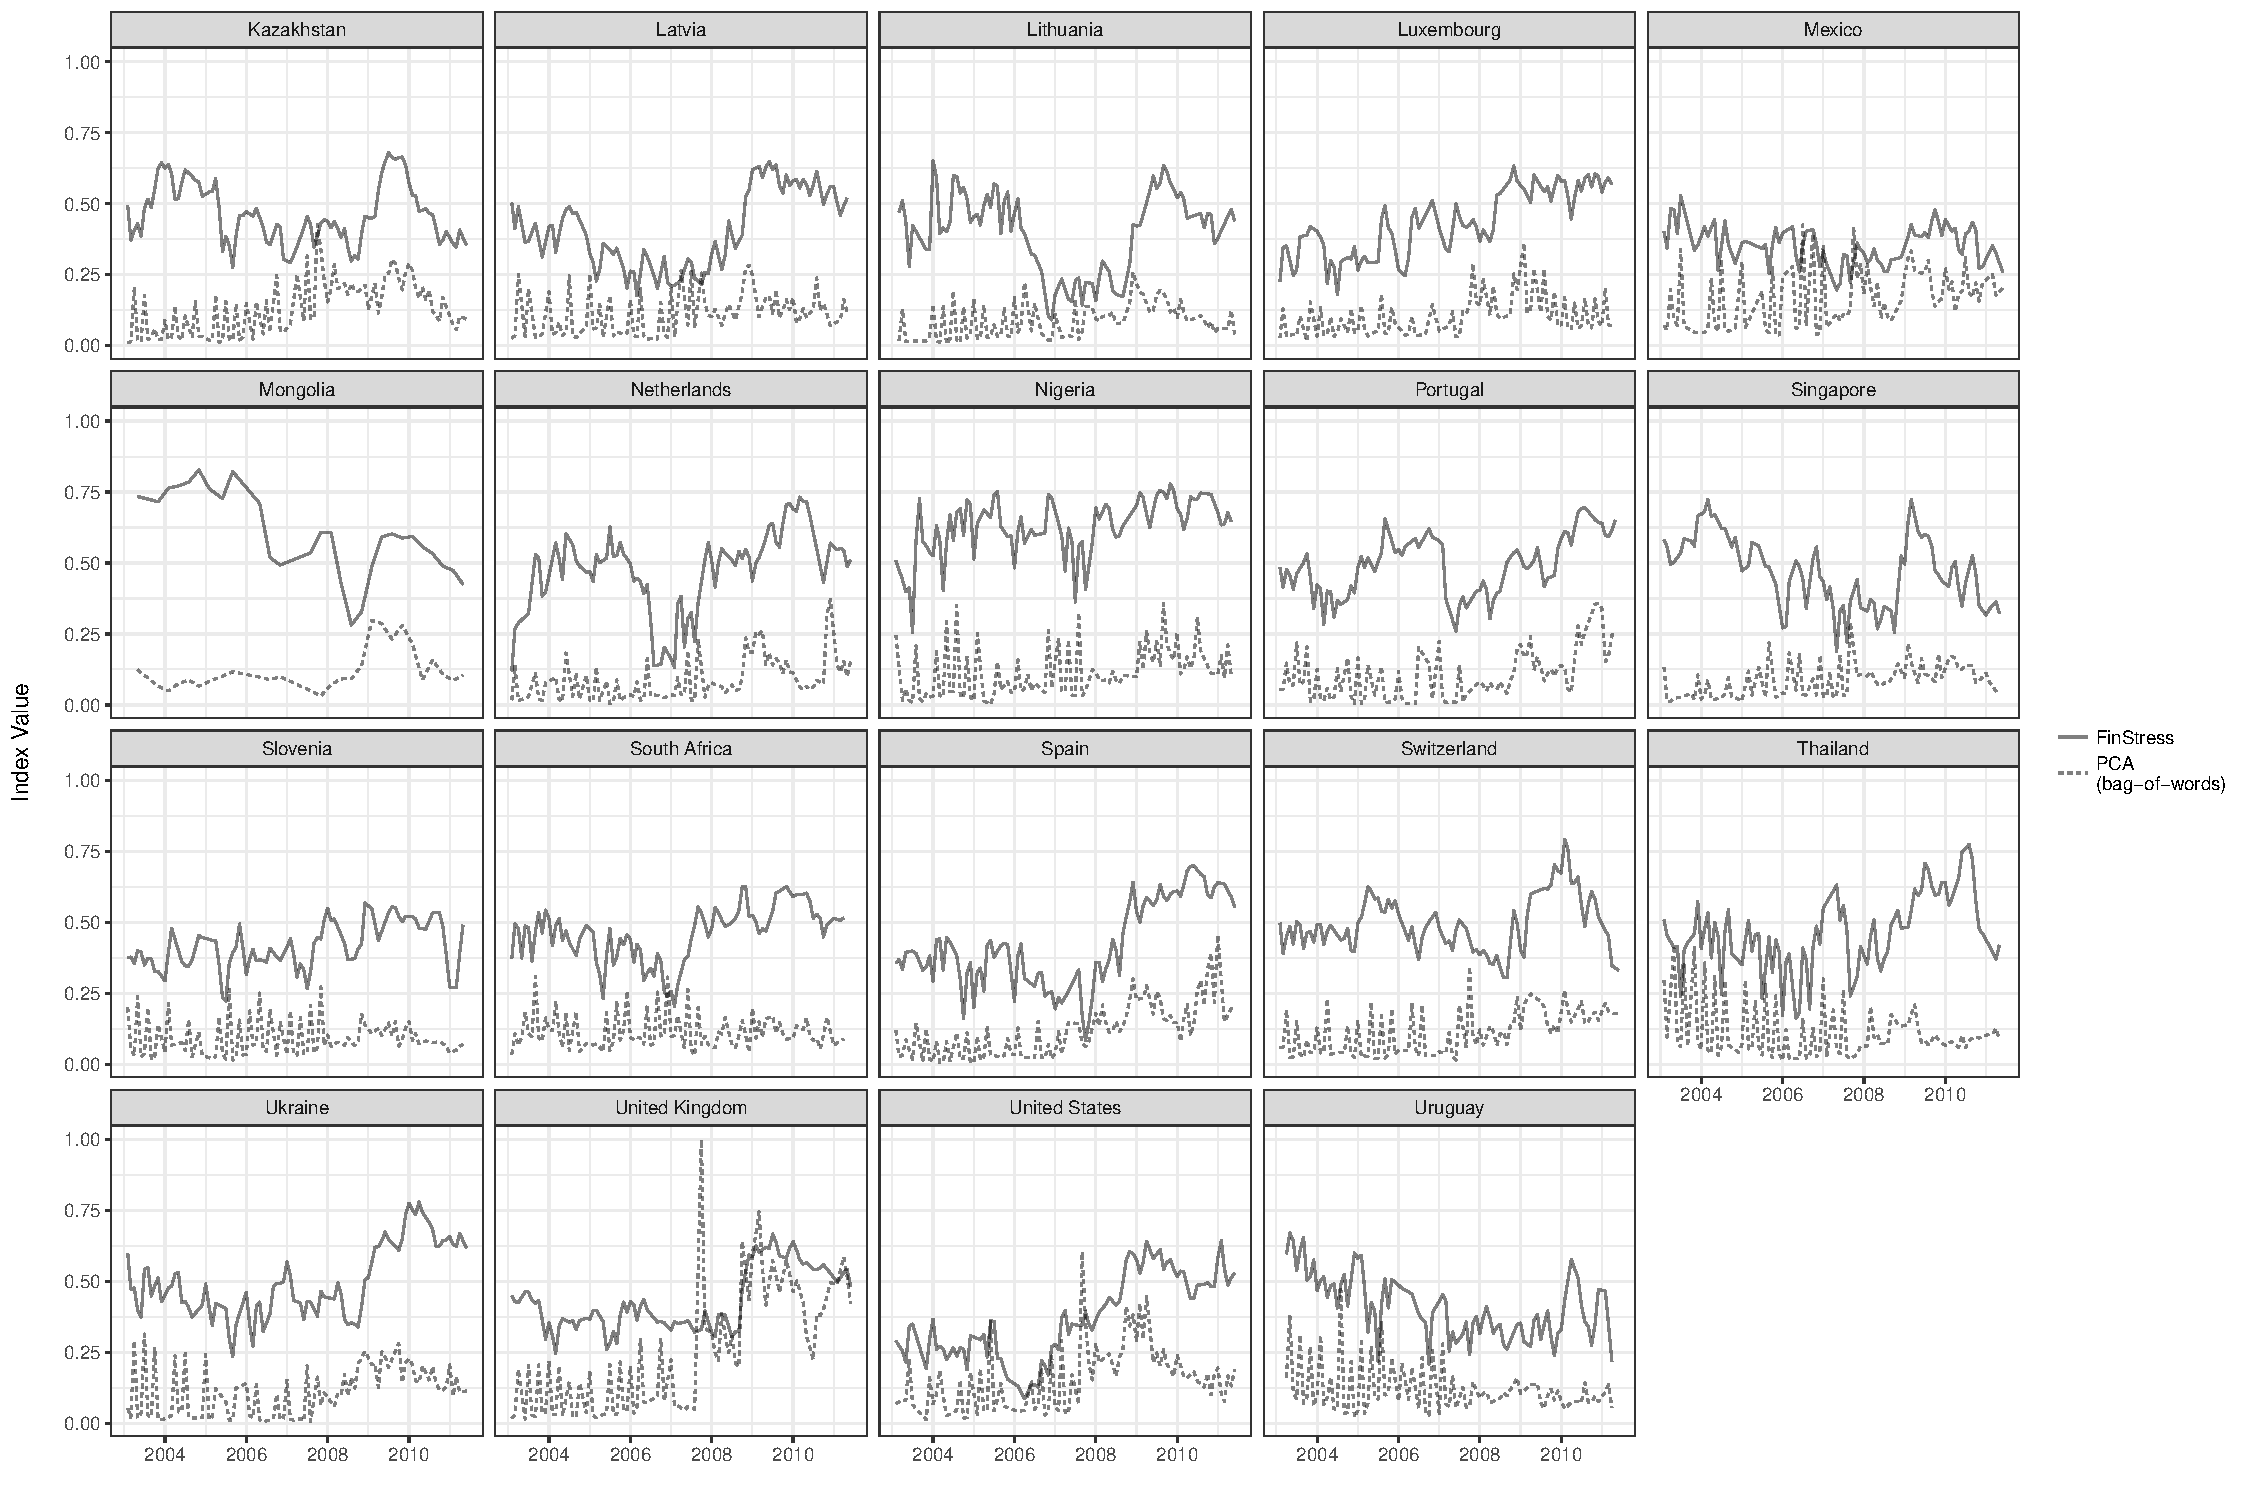
\includegraphics[scale=0.4]{figures/compare_to_pca_2.pdf}
    \end{center}
\end{figure}


\subsection*{FinStress validity: sensitivity to sub-string kernel length}

Previous work using KPCA on English-language texts suggests that sub-string kernel lengths of four to seven characters long are ideal \citep{lodhi2002}. Following this finding, as well as precedent set by \cite{Spirling2012}, we estimated FinStress using five character kernels. We also ran models with three, four, and six character length kernels to examine how sensitive FinStress was to this choice. Note that all aspects of the analysis, e.g. pre- and post-processing were the same across all of these estimations. The first three panels from the top-left in Figure \ref{altKPCA} compare the alternative estimations. There are not meaningful differences between estimates made with four, five, and six character kernels. The estimates using three string kernels--a length below the range suggested by \cite{lodhi2002}--are somewhat different from FinStress. Nonetheless, the estimates are similar overall. We have no reason to believe that kernels shorter than those suggested by the literature are more accurate than our 5 character kernels. It appears from this analysis, that FinStress estimates are not being unduly influenced by our choice to use five character sub-strings rather than other specifications within the range suggested by the literature.

\begin{figure}
	\caption{FinStress--Five Character Kernel PCA--Compared to Alternative KPCA Specifications}
    \label{altKPCA}
    \begin{center}
    	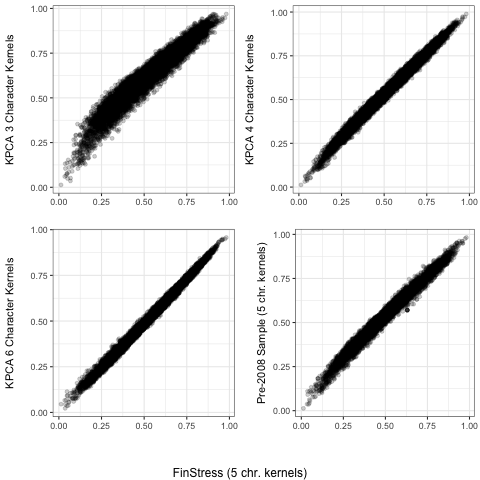
\includegraphics[scale=0.5]{figures/kpca_n_lenth_compare.png}
    \end{center}

\end{figure}

\subsection*{FinStress validity: sensitivity to sample period}

How sensitive are the FinStress estimates to the particular time period included? We discussed in the text how large changes in document style can affect the results. This is why we use only EIU documents from 2003; they follow a consistent style. Similarly are the FinStress results driven by a particular time period due to certain words or types of events in those periods? Do descriptions of future events, such as bursting housing bubbles from 2008 affect how these topics shape FinStress for earlier periods in ways that would not reflect how actors at these earlier times viewed them?

To assess these issues we re-ran KPCA using exactly the same procedures, but only including documents from the 2003 through 2007 period before the start of the Global Financial Crisis. The bottom-right panel of Figure \ref{altKPCA} compares these to the original FinStress results for the same period. They are very similar. This indicates that future events are not unduly influencing past perceptions and that it would be possible to use the KPCA method to extend the analysis using similarly formatted documents from the EIU.


\subsection*{FinStress validity: additional qualitative examinations of texts}

To get a qualitative sense of FinStress' wider qualitative validity, we examined texts associated with minimum and maximum FinStress scores for a number of other countries. Figure \ref{text_selections_max} shows maximum scores for Brazil, Latvia, and Ireland. Brazil had a maximum FinStress score in the sample of 0.65 in 2009. The score reflects the EIU's assessment that the global financial crisis presents risks for banks and lenders ``will find it increasingly difficult to roll over credit lines''. Latvia had a similar maximum FinStress score--0.65 in 2010--and the text this score is generated from clearly describes a  troubled financial sector as it notes that the Bank of Latvia ``appears worried that commercial banks are reluctant to extend new loans''. Ireland had an even higher maximum FinStress score--0.84 in 2011. The text this score is estimated from describes a highly troubled banking system that is going through a painful restructuring process and is reducing the supply of credit to the economy.

The texts that created country-minimum FinStress scores--shown in Table \ref{text_selections_min}--describe ``confidence in financial markets'' in Brazil (2005), ``lending continues to expand'' in Latvia (2006), and stable currency conditions in Ireland (2004). Importantly, in the Brazilian case the text is not without  concerns that the conditions may not continue into the future. All of them (apart from Ireland which was in the Euro and so had monetary policy set by the European Central Bank), mention monetary policy moves to curb overheating. So, while low FinStress scores appear to be reflecting financial markets with strong credit provision, embedded in these texts is a concern that the boom may be peaking. This is an important finding to keep in mind when interpreting the substantive meaning of low FinStress scores. It is an issue that [WITHHELD FOR BLIND REVIEW] formally model in separate work and are able to empirically test using FinStress.

\begin{table}
    \caption{Portions of Texts EIU Reports with Country-\textbf{Maximum} FinStress values (selected countries)}
    \label{text_selections_max}
    	\begin{center}
        \begin{tabular}{c c c | m{10cm}}
            \hline
            Country & Month-Year & FinStress & Text Selection \\
            \hline\hline
            Brazil & August 2003 & 0.58 & While domestic lending to industry picked up in the second half of the year, consumer credit has been flat \ldots the effects of exchange rate depreciation on input costs in 2002 is still being felt in continued pressure on consumer prices in early 2003, requiring stringent monetary policy to suppress inflation. \\[0.5cm]

            Latvia & June 2009 & 0.65 & The economy is slowing sharply, and real GDP contracted by 18\% in the first quarter of 2009 \ldots In the current economic climate most Latvian households and companies will concentrate on reducing their debts; foreign banks operating in Latvia are also trying to reduce their exposure to Latvia by lending less. \\[0.5cm]

            Ireland & April 2011 & 0.78 & Irish households are highly indebted. Private consumption will therefore be constrained as households rebalance their balance sheets and as credit conditions remain tight in 2011-13. Investment will continue to shrink in 2012 as the collapse of the construction industry maintains momentum \ldots [the] most recent stress tests reveal the complete failure of earlier attempts to assess the impairment of the banks' balance sheets. Of particular note is the fact that no serious provision had previously been made for losses on the banks' mortgage lending, despite a massive collapse in the residential property market that has been ongoing for some years. \\[0.5cm]


            \hline
    \end{tabular}
    \end{center}
\end{table}


\begin{table}
    \caption{Portions of Texts EIU Reports with Country-\textbf{Minimum} FinStress Values (selected countries)}
    \label{text_selections_min}
    	\begin{center}
        \begin{tabular}{c c c | m{10cm}}
            \hline
            Country & Month-Year & FinStress & Text Selection \\
            \hline\hline
            Brazil & August 2005 & 0.05 & By continuing to meet the target for the primary fiscal surplus despite strong political pressure to increase spending on social programmes, and by increasing the benchmark Selic overnight rate until inflation began to subside in June, the government has confirmed its cautious stance. Apart from keeping a rein on inflation, this has helped to maintain confidence in the financial markets. \\[0.5cm]

            Latvia & March 2006 & 0.18 & The BoL [Bank of Latvia] has tried to curb the current lending boom by raising the mandatory reserve requirements for banks from 4\% to 8\% in 2005, in two steps. Further increases seem unlikely, as Latvian customers could be served from other EU countries if the costs of banking in Latvia become excessive. \\[0.5cm]

            Ireland & January 2007 & 0.06 & Private consumption will be fuelled in 2007 by strong employment growth, solid real wage increases, tax cuts, lower inflation and the maturing of a generous government-financed savings scheme \ldots Strong business confidence and a still-booming construction sector will bolster growth, but an anticipated cooling of the housing market will account for the deceleration over the outlook period. \\[0.5cm]


            \hline
    \end{tabular}
    \end{center}
\end{table}


\subsection*{Developed vs.~developing
countries}\label{developed-vs.developing-countries}

Developing countries often lack strong financial institutions and systems. Facing a very risky pool of borrowers, banks tend to make fewer loans \citep{Andrianova2014}. So we should expect them to face generally tighter credit market conditions than developed countries.

The left panel of Figure \ref{comp_dev_developing} shows average stress levels in developed vs. developing countries that Laeven and Valencia code as not being in crisis--indicates that there is a difference in the level of perceived financial market stress in developed and developing countries from 2003 to 2008. Developing countries on average have higher FinStress scores. For example, the mean score in middle and low income countries (as classified by the World Bank) is 0.55 in 2005, a level developed countries only reached after the collapse of Lehman Brothers in 2008.\footnote{The 2005 mean for high income countries is 0.47} The mean levels across the two groups converge in the Global Financial Crisis. The distribution of FinStress scores in these two groups of countries across the sample is significantly different in the expected direction in the sample using one-sided Kolmogorov-Smirnov tests.\footnote{We ran the tests using the \texttt{ks.test} function from base R.}

Nonetheless, during periods that the binary Laeven and Valencia measure codes as being a crisis, i.e. implement policy responses to financial market stress,the two sets of scores are very similar (see the right-panel of Figure \ref{comp_dev_developing}). Apart from 2007 and 2008 where the binary measures have significant ``annual rounding error'',\footnote{Remember that the binary measure can include both less and more stressed portions of a year as all being in crisis.} on average countries in crisis have FinStress scores above about 0.55. It appears that while developed countries have more stressed financial markets than developed countries that on average, developed and developing countries have clear policy responses to financial market stress when their FinStress scores are well above about 0.55.

\begin{figure}
    \caption{Comparison of Mean FinStress Scores in High vs. Low and Medium Income Countries}
    \label{comp_dev_developing}

    \begin{center}
        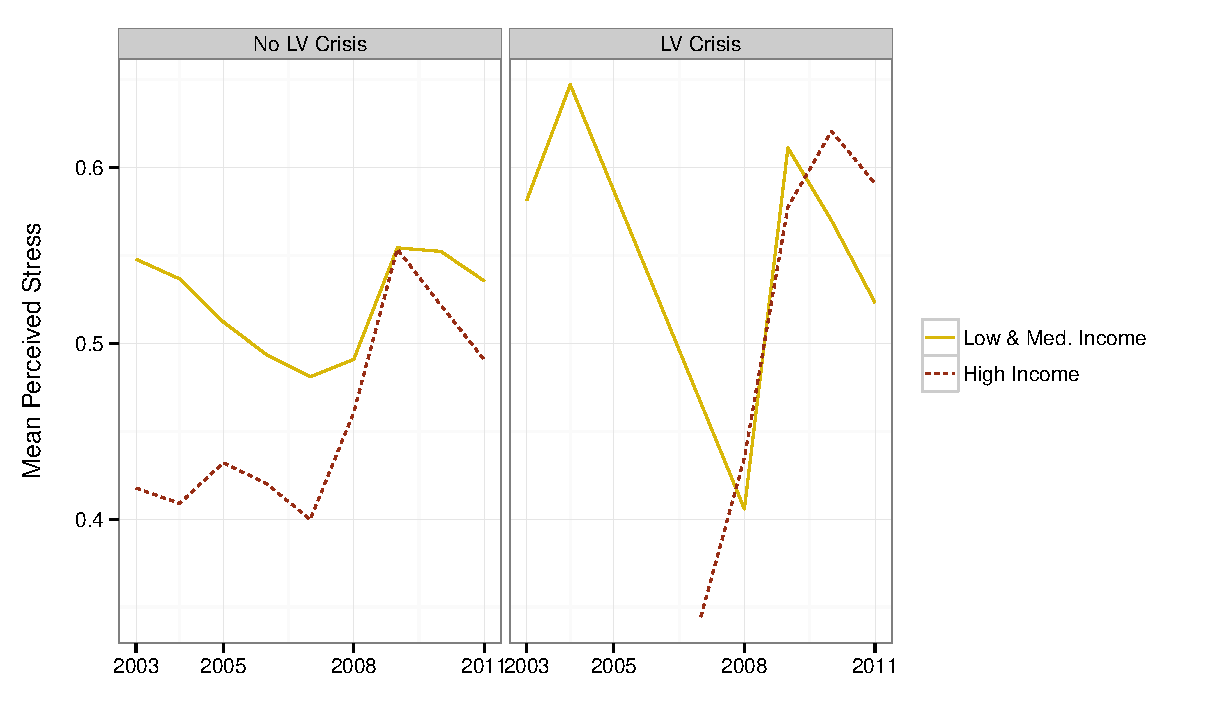
\includegraphics[scale=0.55]{figures/dev_vs_developing.pdf}
    \end{center}
    {\scriptsize{Plot excludes Uruguay, which was a substantial outlier with a much lower average FinStress score during what Laeven and Valencia classify as a crisis than all other developing countries.}}
\end{figure}

\subsection*{Correlations Between FinStress and Camel Variables}

How does FinStress correlate with the components of the CAMELS system of bank soundness? We used annual FinStress means to compare it to annual national aggregates of the CAMELS variables in \cite{Andrianova2015}. Figure \ref{camel_plot} shows the bi-variate relationships between FinStress and these variables. FinStress is statistically significantly associated with six of the seven CAMELS variables at the 5 percent level.\footnote{It is not significantly associated with Return on Average Assets.} FinStress is strongly associated with three of the CAMELS variables in that there is a correlation coefficient greater than 0.2 or less than -0.2. These variables are impaired assets to gross loans, net loans to total assets, and liquid assets to total assets. See also Figure \ref{cor_camel} for the full correlation matrix. FinStress is most strongly positively associated with impaired assets.\footnote{The log of impaired assets--it is a highly skewed variable--is associated with FinStress with a correlation coefficient of 0.45, significant at all standard levels}

\begin{figure}
	\caption{Comparing Annual Mean Perceptions of Financial Market Conditions with Components of the CAMELS System from \cite{Andrianova2015}}
    \label{camel_plot}
    \begin{center}
		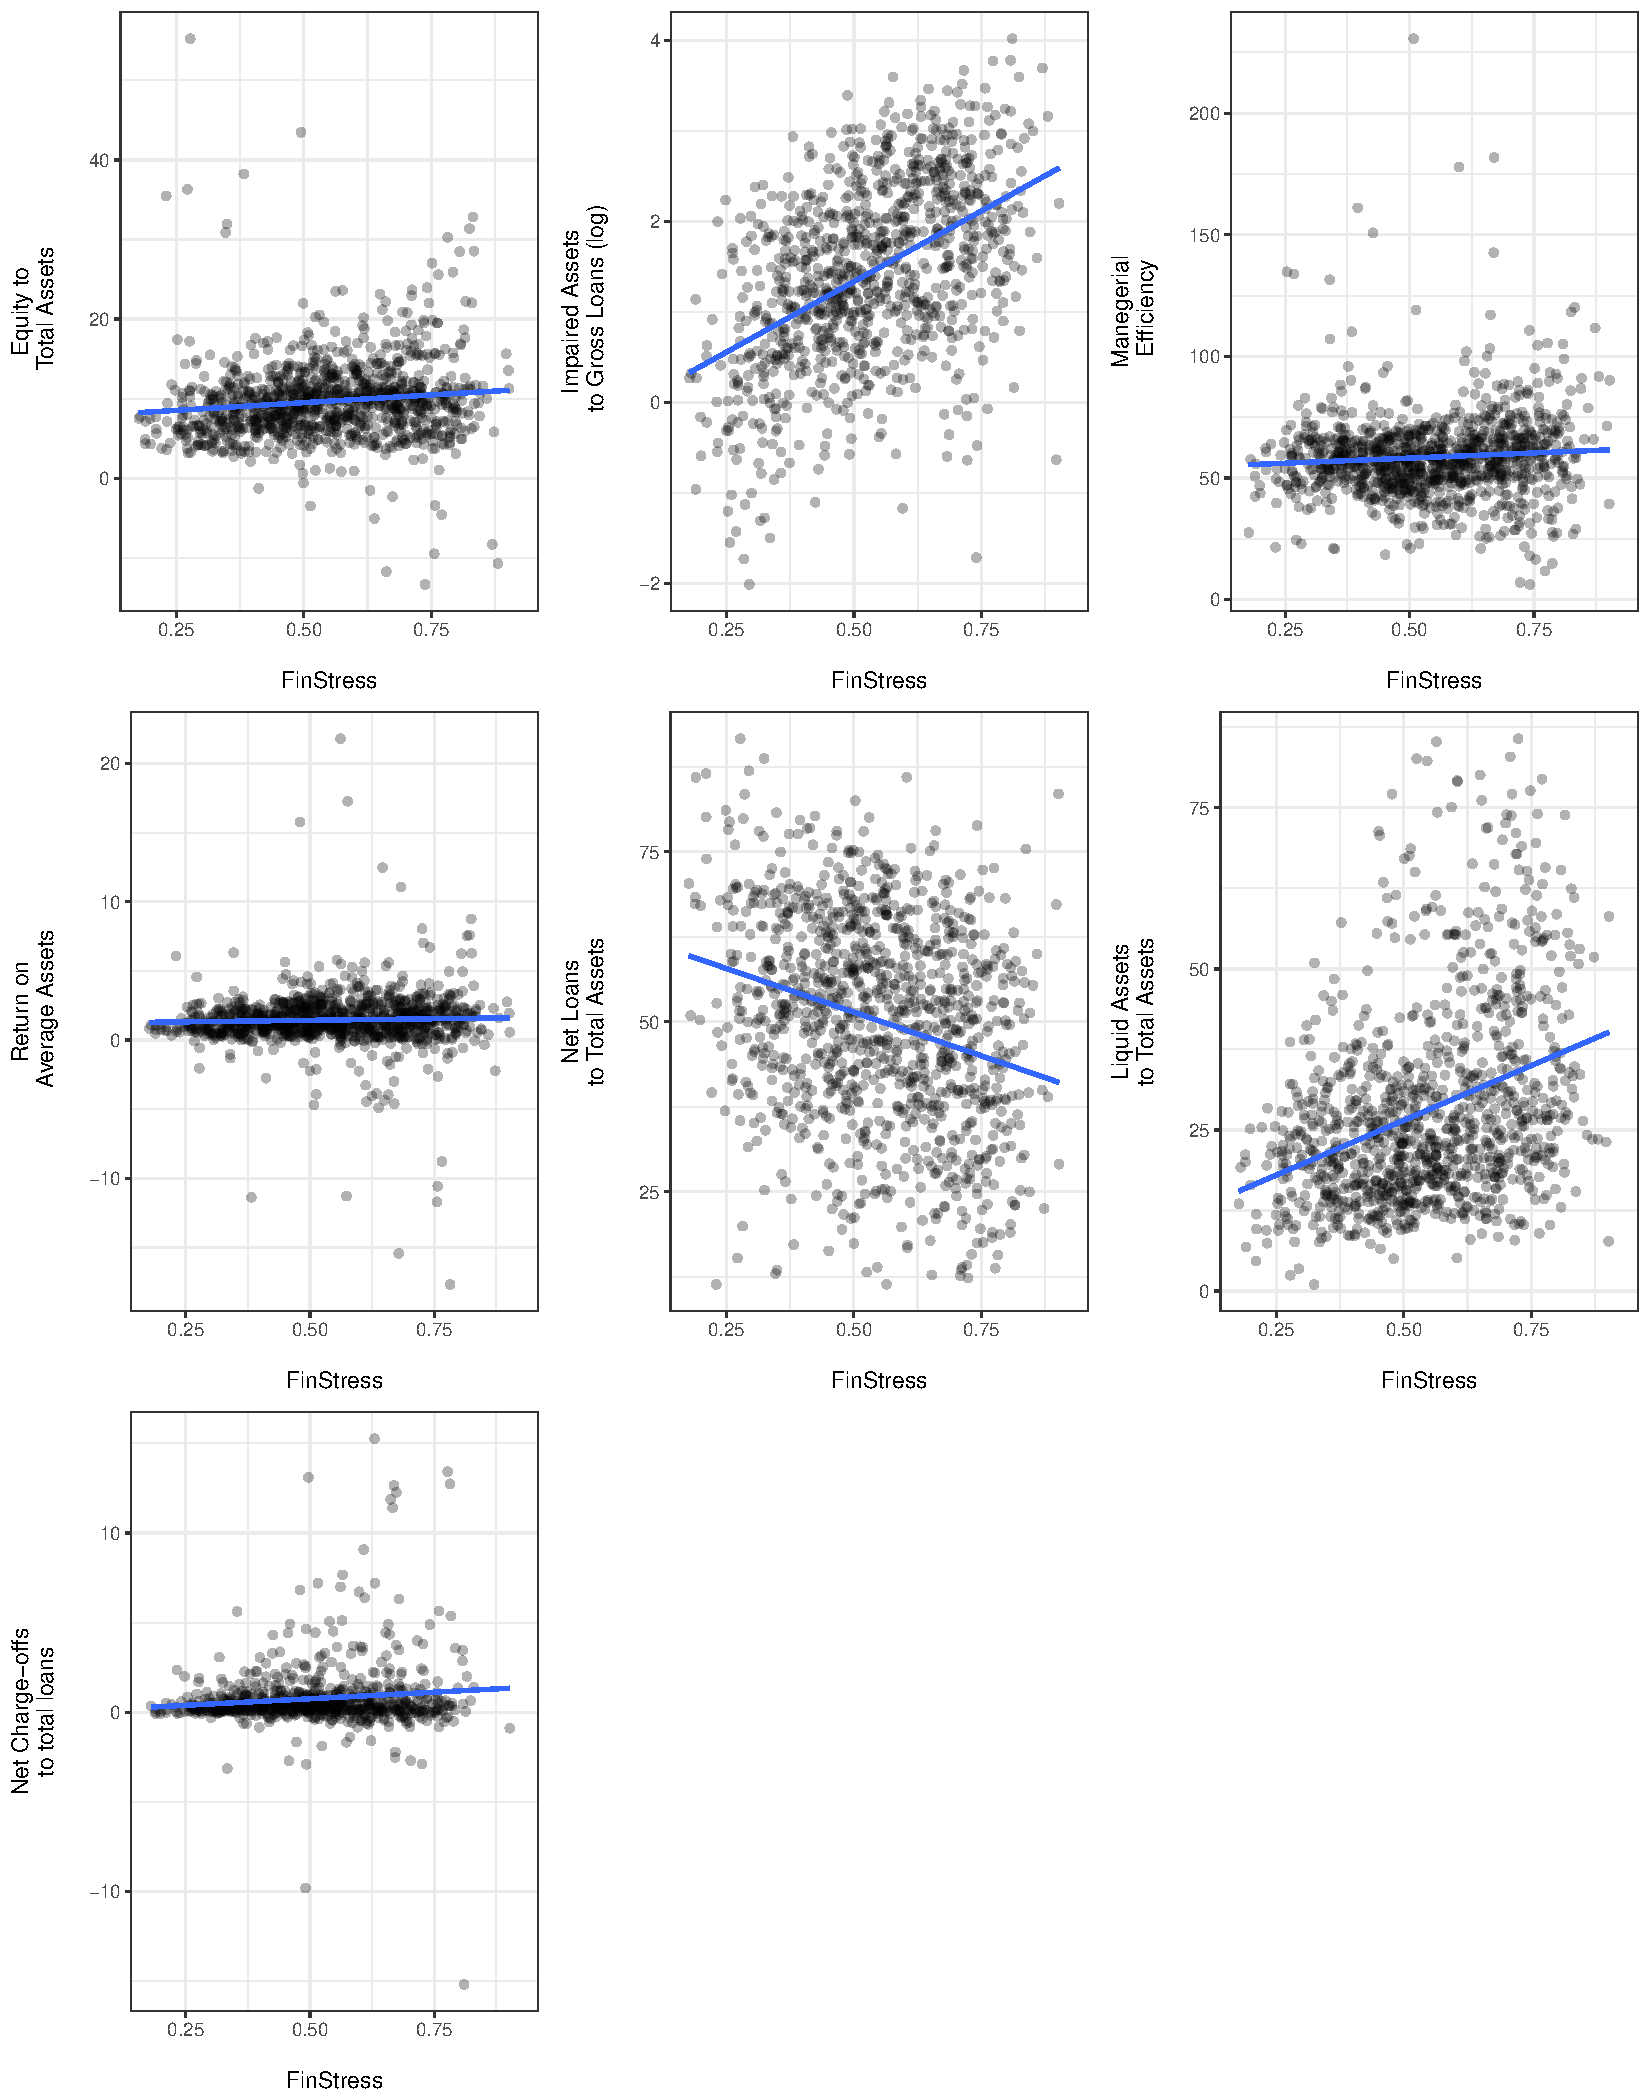
\includegraphics[scale=0.55]{figures/fin_fragility_compare.pdf}
	\end{center}
\end{figure}

\begin{figure}[H]
	\caption{Correlation between Annual FinStress Mean Scores and CAMELS Variables from \cite{Andrianova2015}}
    \label{cor_camel}
    \begin{center}
    	\includegraphics[scale=0.5]{figures/ff_corr_matrix.pdf}
    \end{center}
\end{figure}

\subsection*{Global comparison to accounting measures of banking system fragility}

Moving beyond simple correlations, to assess the relationships between the various quantitative measures of bank and banking system stress and FinStress we use a random forest regression. We include in the regression CAMELS indicators from \cite{Andrianova2015} and a number of other indicators from the Global Financial Development Database that the World Bank classified as being related to banking system stability \citep{worldbank2015}, including Z-Scores.\footnote{Variables from the GFDD include: provisions to NPLs, stock price volatility, regulatory capital to assets, capital to assets, credit to deposits, stock market returns, and private sector credit provided by banks and other financial institutions. The last two are not classified by the GFDD as banking ``stability'' indicators, but we included them as they may be substantively important.} Our main reason for using random forest regressions is that we are examining the relationships between many highly correlated variables and FinStress. As all of the right-hand side variables are country-year aggregates, we examine their relationship with country-year mean FinStress levels.

The random forest regressions are based on a slim sub-sample for which we have FinStress scores. There are 1,677 country-years for which we have average FinStress scores, but due to missingness issues discussed above, only 425 of these have complete information across the included indicators and thus are included in the random forest regression.

Figure \ref{rf_var_importance} shows the importance each variable plays on average for predicting FinStress levels. Impaired loans are found to be the most important variable for predicting FinStress levels in this sub-sample.\footnote{In a sample of all countries, exchange rate change is also relatively important, though when the sample is subsetted to look only at high income countries, it has no impact on reducing predictive error. This makes substantive sense as in the period under examination exchange rates in high income countries were relatively stable, even during crises. Stress in developing countries is closely related to foreign exchange disruptions and the currency asset-liability mismatches banks face in these situations.} The third most important is highly related to impaired assets--return on average assets. When there are more non-performing loans the average return on all loans is lower. Z-Scores are a fairly poor predictor of FinStress. Please see below for a detailed exploration of the relationship between FinStress and Z-Scores. The main conclusion of this work is that Z-Scores, at least as measured by the World Bank, are a poor measure for examining how banking stress changes over time and should be avoided in research on this.

Figure \ref{rf_partial_depend} shows the predicted values from repeated draws of FinStress averaged within the values of the other variables included in the random forest regressions \citep[see][14]{jones2015}. This gives us a window into the nature of the estimated relationship between the predictor variables and FinStress. Impaired loans (log) have an almost linear 45 degree positive relationship with FinStress. Higher impaired loan ratios are strongly associated with higher FinStress scores. Impaired assets are otherwise often known as non-performing loans. Banks are solvent when their assets (e.g. loans and the income they generate) can cover their liabilities (e.g. deposit withdrawals). Impaired assets greatly threaten banks' ability to meet their obligations and so threaten their solvency. As such, it seems as though FinStress is closely related to bank balance sheet health.

Greater stock price volatility also appears to have a strong linear relationship with FinStress, where more volatility is related to higher FinStress scores. While most of the other variables appear to have less linear relationships with FinStress, they are generally in the expected direction. For example, the higher banks' return on average assets, the higher their equity, and the higher their provisioning, the lower the FinStress scores. These findings further corroborate the proposition that FinStress is a valid indicator of financial market stress, specifically in banking, and give more definition to specifically what the Index measures.

Finally, it is important to examine the perhaps initially counter-intuitive finding that FinStress is positively associated with liquid (e.g. cash) asset ratios. Banks with more liquid assets are less likely to become insolvent because they can use these assets to meet their liabilities. However, high liquid asset ratios can be a manifestation of a stressed financial system as banks create large liquid asset stockpiles when they are reluctant to lend--take on less liquid assets. This behavior restricts credit to the wider financial system and economy. Following the Lehman Brothers collapse in 2008 an extreme version of this occurred, becoming known as a ``credit crunch''. \cite{Andrianova2014} find that African banks have very high liquid asset ratios because lending risks are high, so banks are reluctant to make new loans. This may explain why developing countries often have persistently high FinStress scores (see above). To a large extent net loans and liquid assets are inversely related. As such we find a negative relationship between net loans and FinStress--banks in countries with higher FinStress scores are making fewer loans and instead are hoarding liquid assets.

\begin{figure}
    \caption{Importance of Various Quantitative Financial System Stability Measures for Predicting EIU Perceptions of Financial Market Stress Index}
    \label{rf_var_importance}
    \begin{center}
        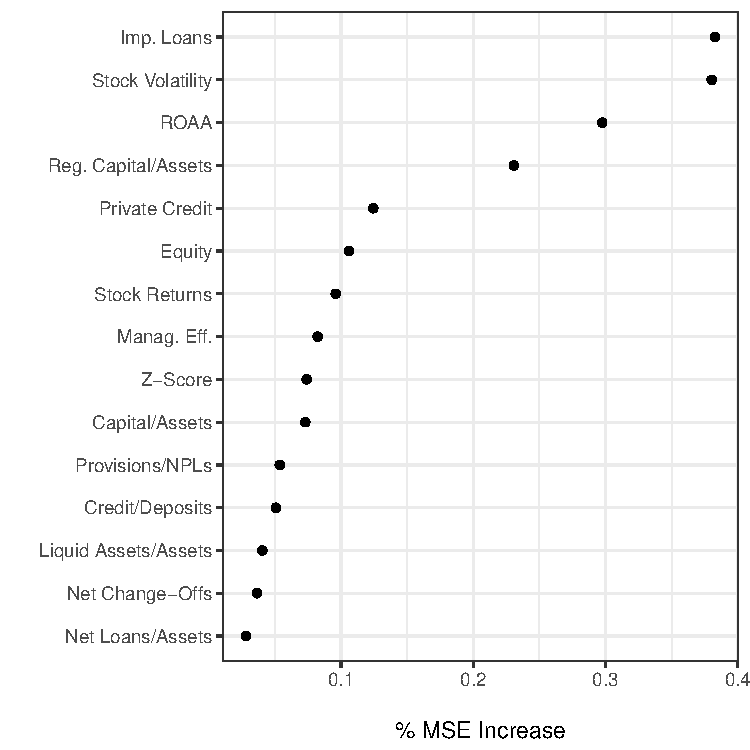
\includegraphics[scale=0.5]{figures/rf_variable_imp.pdf}
    \end{center}
\end{figure}

\begin{landscape}
\begin{figure}
    \caption{Partial Dependence of Each Predictor in the Random Forest Regression on FinStress ($\hat{y}$)}
    \label{rf_partial_depend}
    \begin{center}
        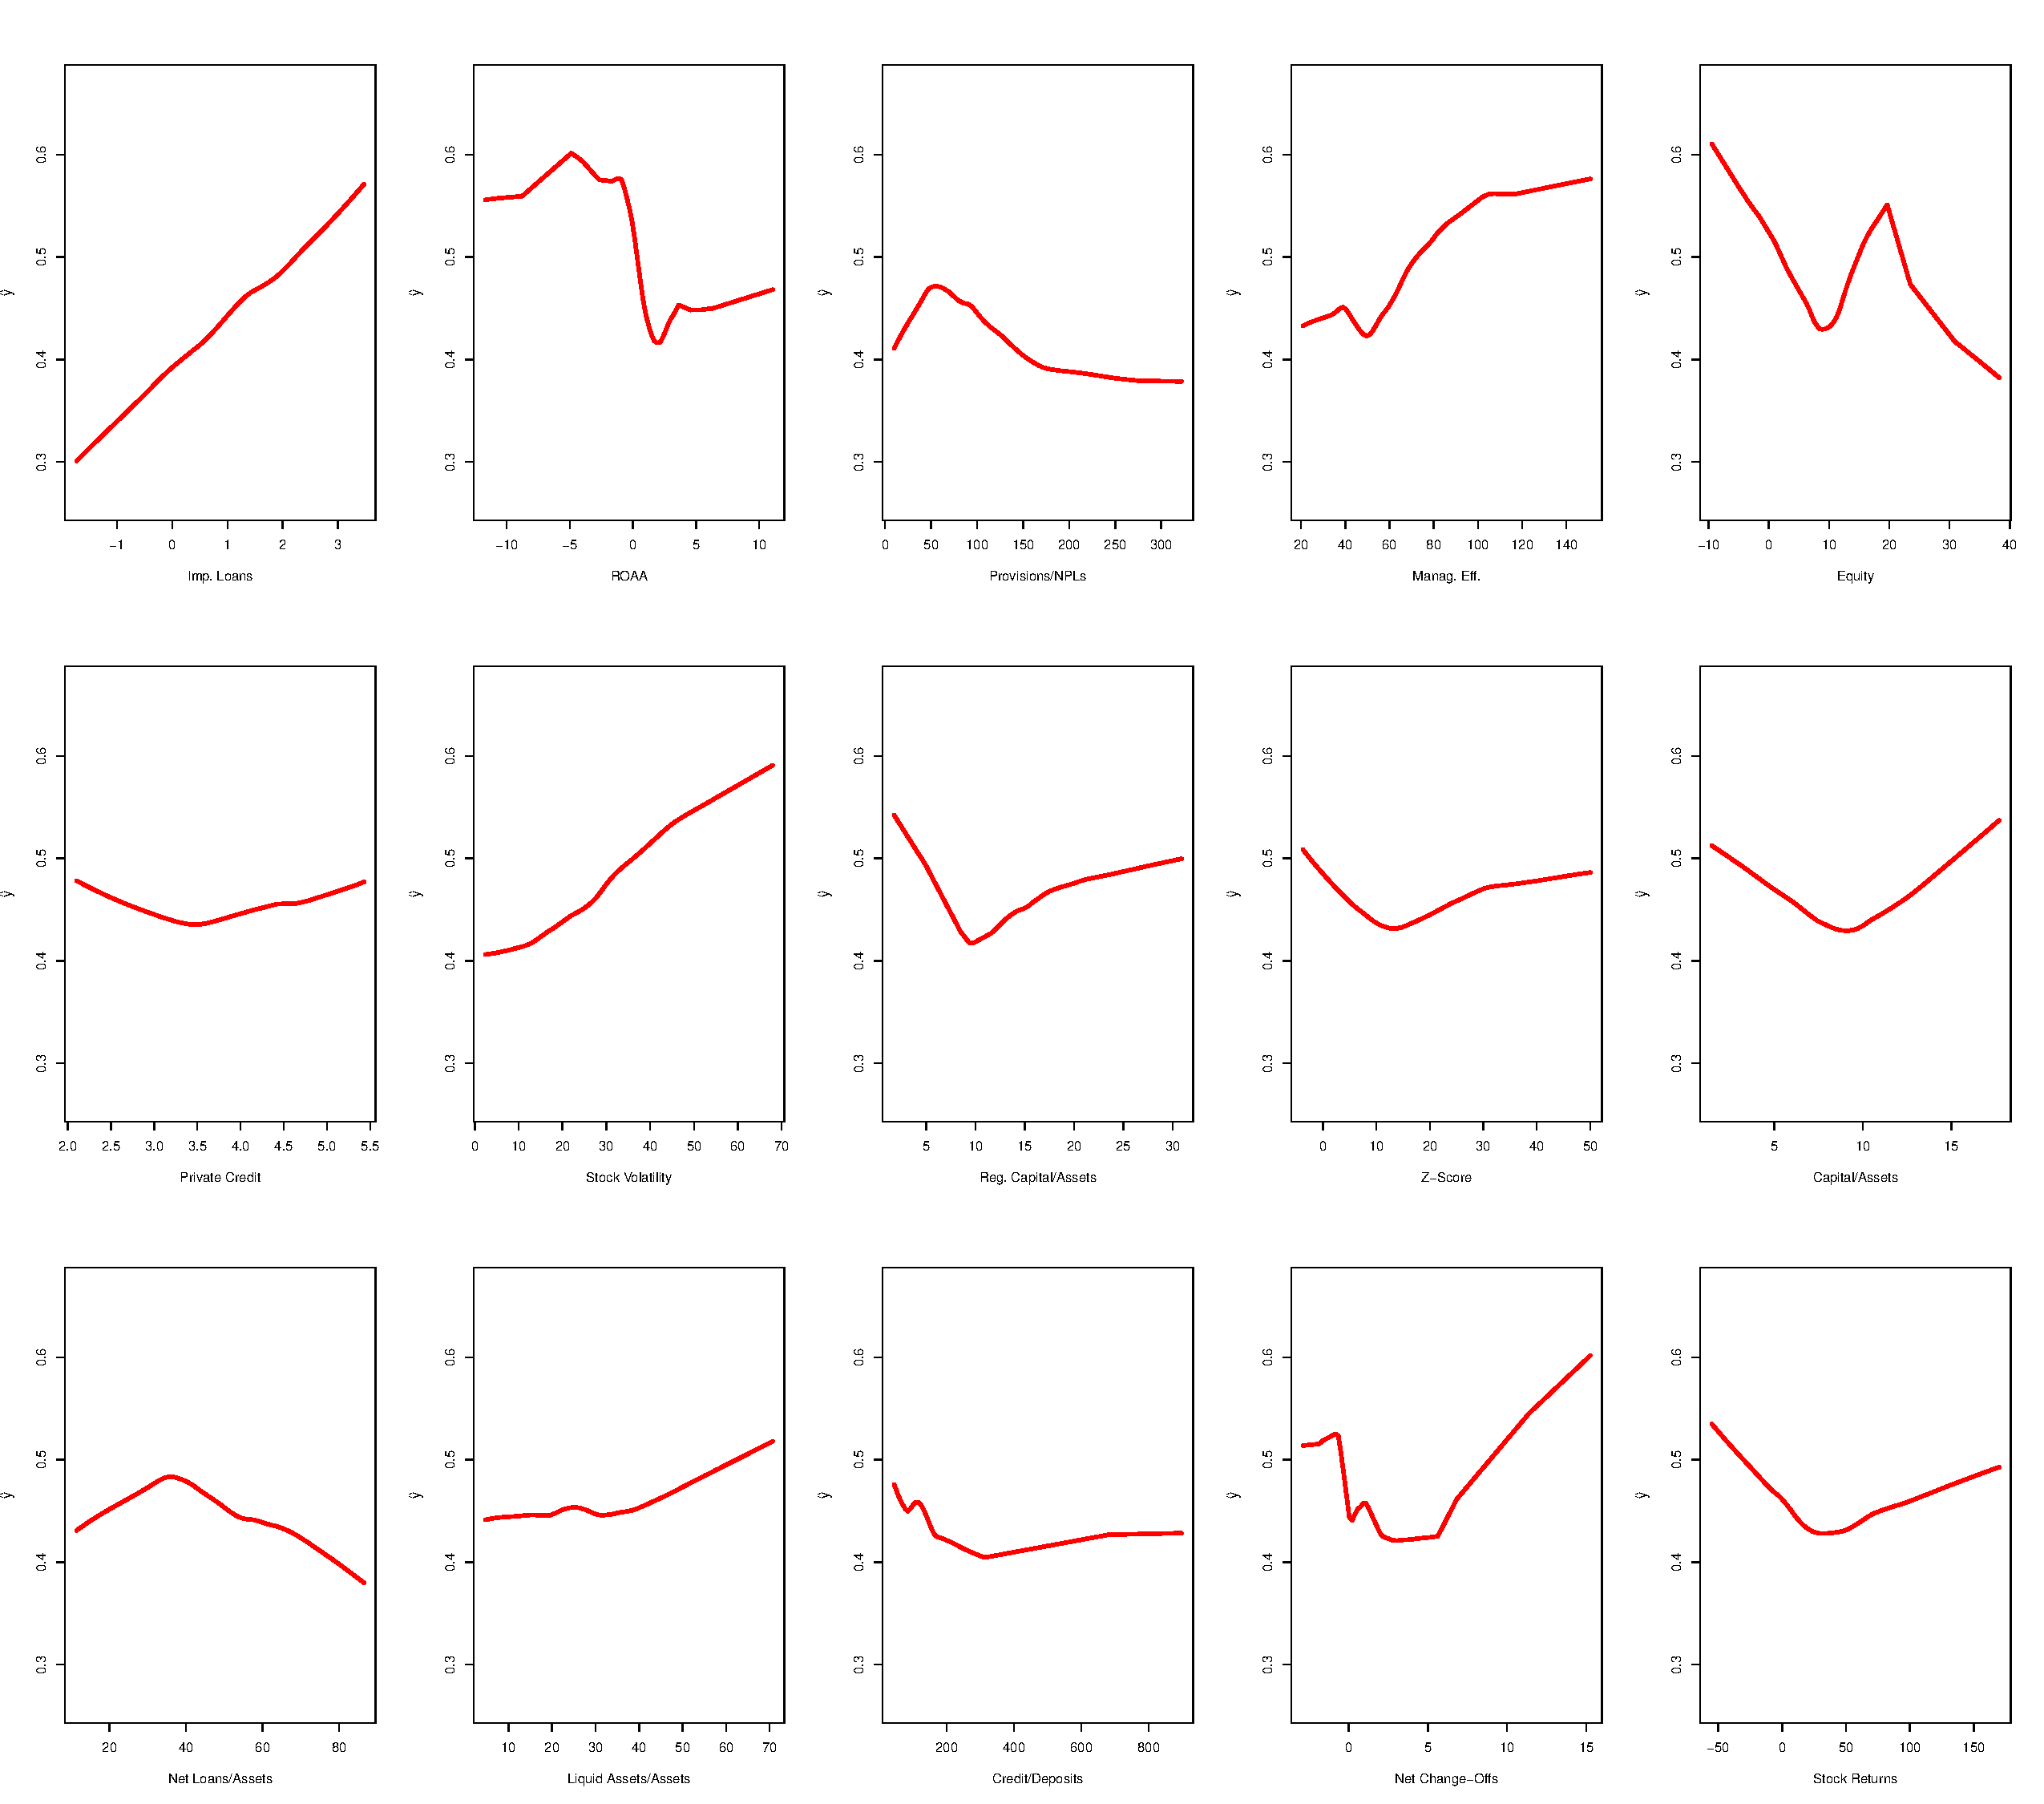
\includegraphics[scale=0.42]{figures/rf_partial_dependence.pdf}
    \end{center}

\end{figure}
\end{landscape}


\subsection*{FinStress compared to Z-Scores}

How does FinStress compare to the widely used Z-Score measure of banking system fragility? We saw in the main text that the global random forest regression indicates that Z-Scores are not very predictive of FinStress. Given the prominence of the Z-Score measure in the finance literature, we wanted to further explore this (null) relationship.

It is important to note that the two quantities do measure different phenomena--perceptions for the former and bank accounting relationships for the latter--, but both potentially  provide indications of stress. As was the case for the dichotomous measures of financial crises, we would expect them to be positively correlated with one another. Another interesting question would be whether one would precede the other. Does weakness in accounting quantities proceed perceived stress?

To explore these possibilities, we compare FinStress to the easily accessible Bank Z-Score measure compiled from Bankscope data in the World Bank's Global Financial Development Database (GFDD) project \citep{worldbank2013}.\footnote{Indicator ID: GFDD.SI.01. Accessed January 2017.} The measure is interpretable as the inverse of the upper bound of the probability of the banking system's insolvency.\footnote{Formally: $\frac{\mathrm{ROA}_{t} + \frac{\mathrm{equity}_{t}}{\mathrm{assets}_{t}}}{\sigma_{\mathrm{ROA}}}$. $\mathrm{ROA}$ is return on equity. $\sigma_{\mathrm{ROA}}$ is presumably for the entire period for which data is available, though the World Bank's documentation does not explicitly specify this. It is common in other work for the $\sigma_{\mathrm{ROA}}$ to be based on a three year rolling window \cite[225]{beck2013bank}. All quantities are country aggregates.} Figure~\ref{z_score} shows a comparison of the two measures for selected countries. Note that to ease visual comparability we rescaled the Z-Scores to be within zero and one as before, and reversed the scale so that larger values indicate a higher probability of banking system insolvency.\footnote{It is common to log-transform the Z-Scores \cite[225]{beck2013bank}. However, it is unclear how previous work has done this as there are negative values in the Z-score that would create undefined values when logged.} As before, we converted FinStress to yearly averages for comparability.

There does not appear to be much of a relationship between Z-Scores and FinStress. The rescaled World Bank Z-Scores are positively correlated with FinStress, but this is not significant at the 10\% level.\footnote{We also examined an alternative data source compiled by \cite{Andrianova2015}, which transformed Bankscope data as well. In this case there was a weak positive association significant at the 5\% level. However, again there was little cross-time variation in the Z-Score.} Interestingly, the World Bank's Z-Scores do not vary significantly within countries over time, especially compared to  FinStress. There is little difference between Z-Scores for countries during periods of heightened financial stress (however measured) and more stable times. Thus Z-Scores, at least those provided by the World Bank, are not a useful indicator of financial crisis states. Z-Scores do not appear to predict perceptions of financial market stress. In a simple partial correction linear regression that had FinStress as the dependent variable and included lagged FinStress, lagged Z-Scores, and country fixed-effects, Z-Scores were not statistically significantly associated with perceptions of financial market stress (see Table \ref{finstress_z_regress}).

The simplicity with which Z-Scores can be calculated with readily available data likely contributes to their wide use in the literature, especially relative to other quantitative measures of financial system fragility that are often difficult to obtain. However, it is clear that Z-Scores--at least the version available through the World Bank's GFDD--are a sub-optimal cross-time measure of financial market stress. It is beyond the scope of our article to determine the source of the measure's peculiar characteristics, but they are important to note here: the indicator has weak time-variance, it does not distinguish between periods of significant known financial market stress and less stressful times, and it does not help us predict perceived financial market stress. FinStress, in contrast, is much notably time-variant in ways that correspond closely to prior information on financial market stress.

\begin{figure}

    \caption{Annual Mean FinStress Compared to Country-level Z-Scores (rescaled)}
    \label{z_score}

    \begin{center}
        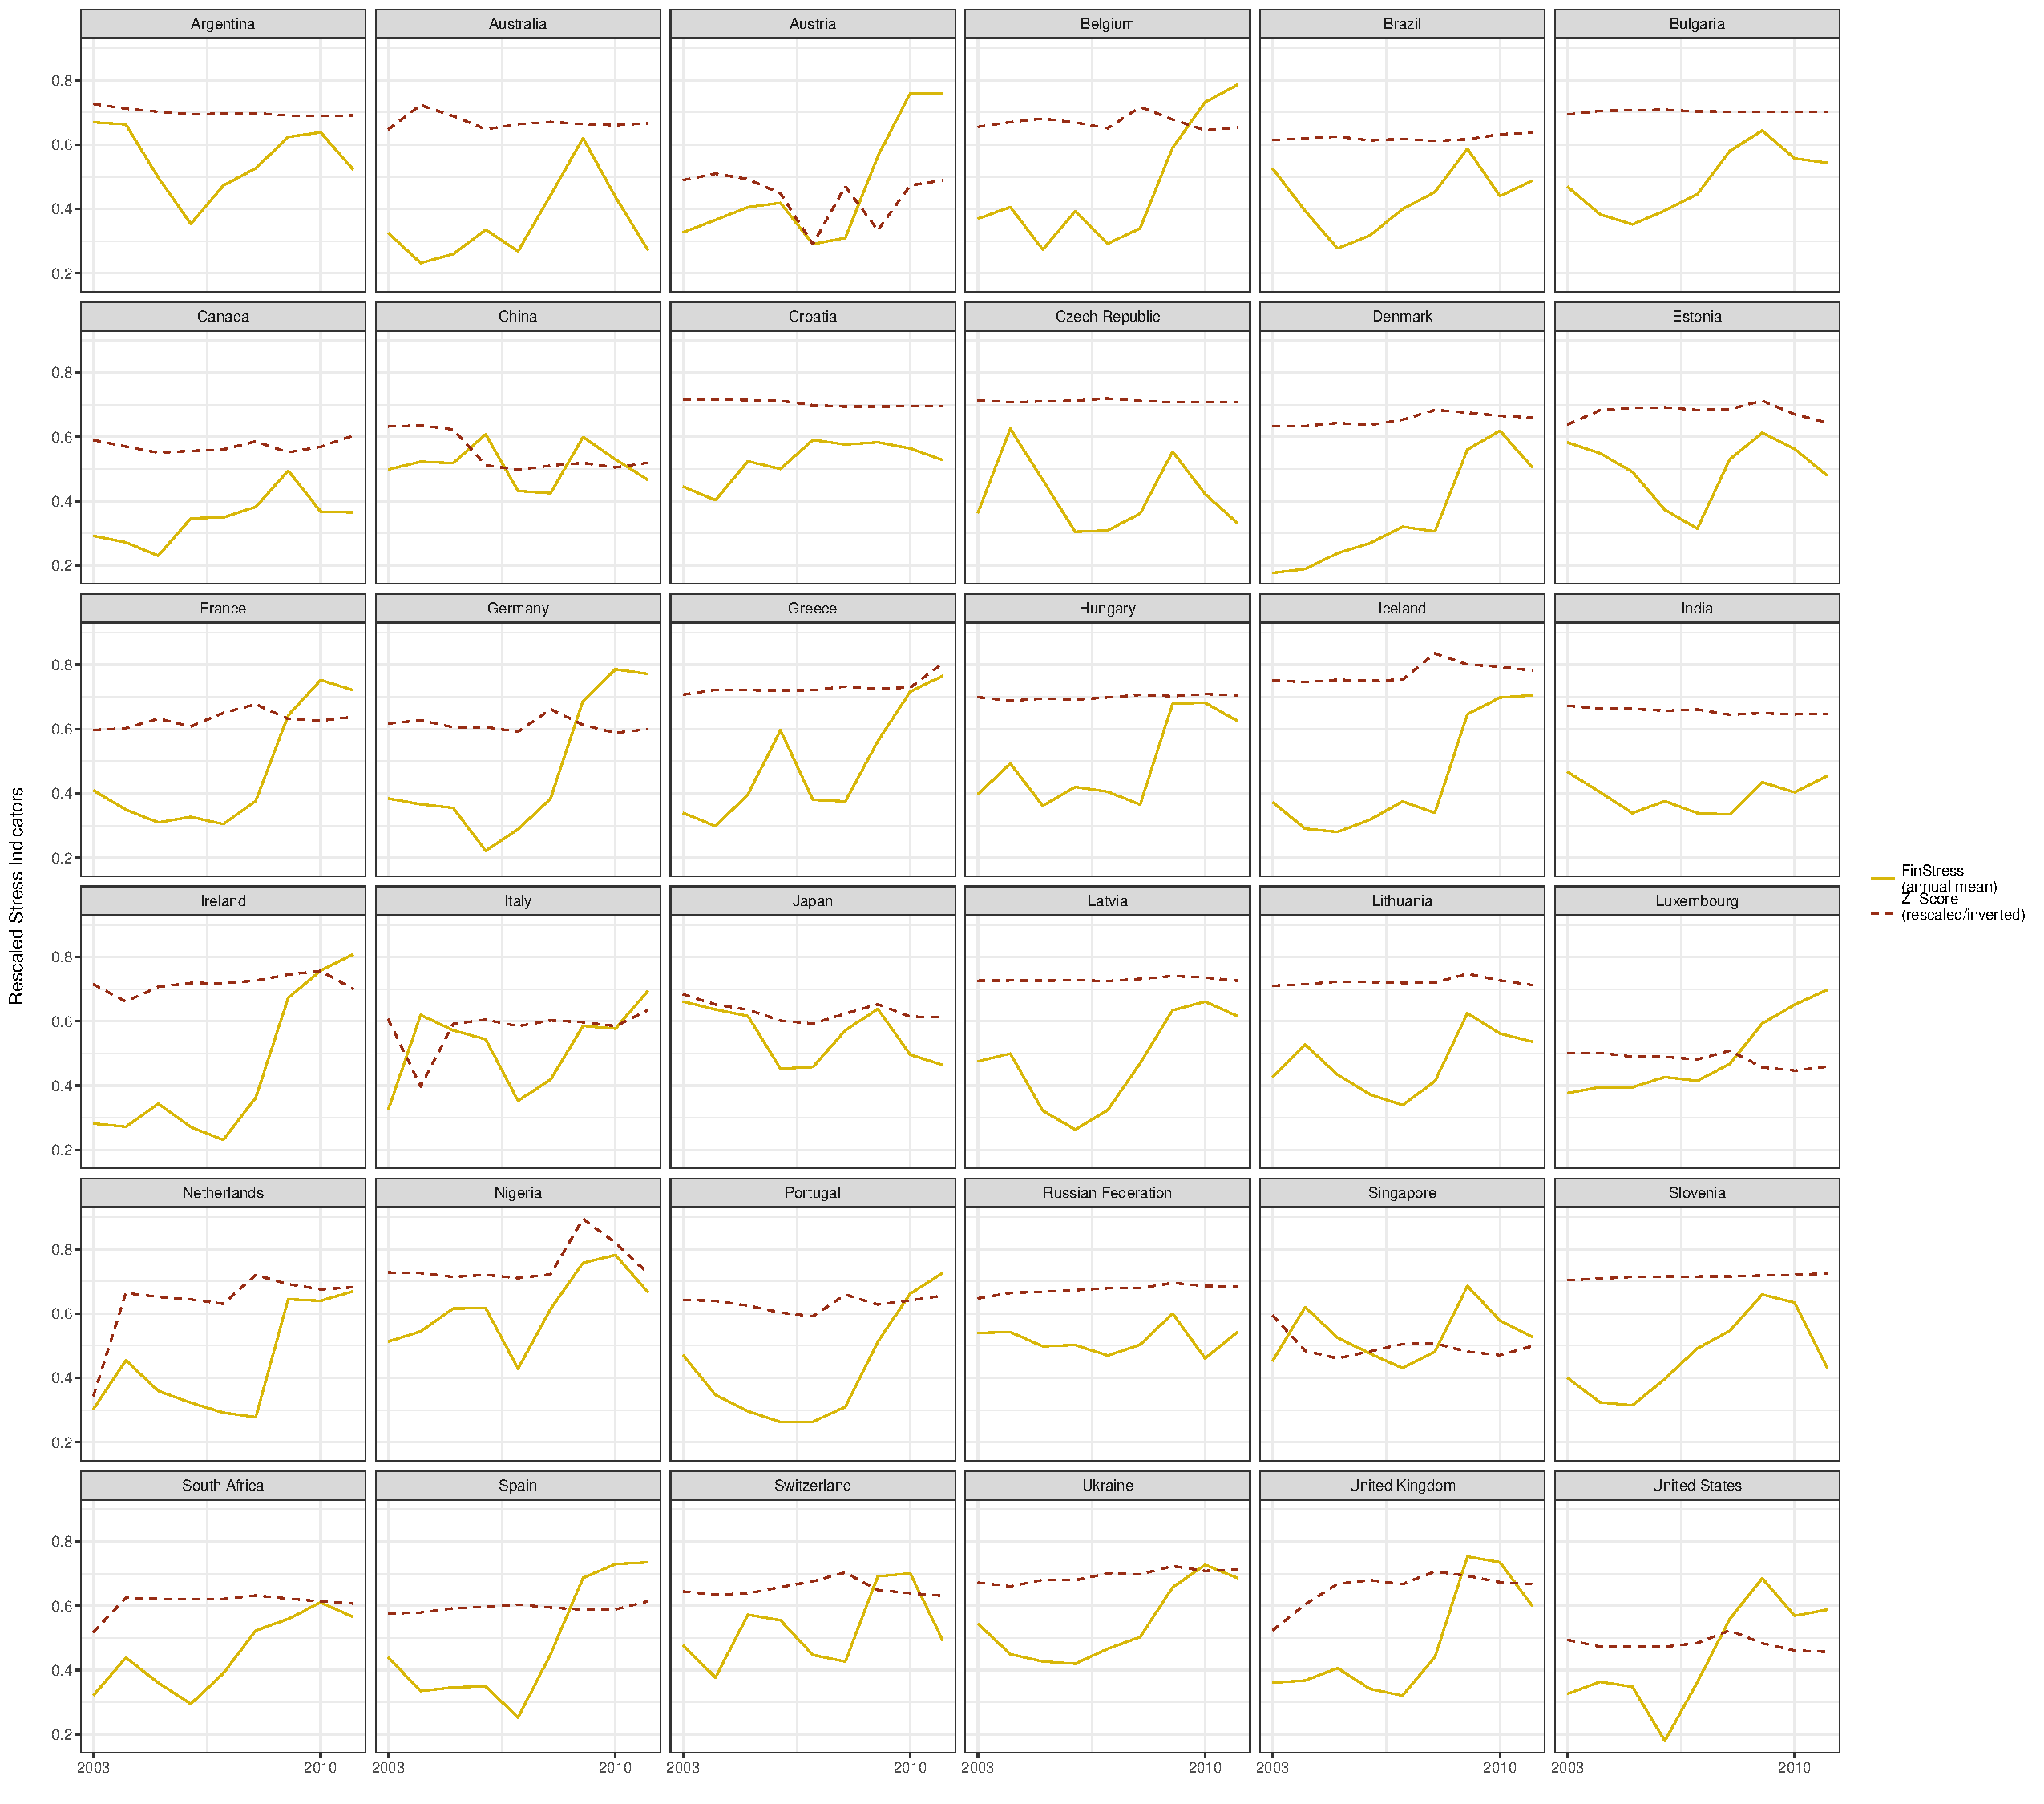
\includegraphics[scale=0.4]{figures/compare_to_z-score.pdf}
    \end{center}

\end{figure}

\begin{table}[H]
    \caption{Do Z-Scores Predict Perceived Financial Market Stress?}
    \label{finstress_z_regress}

    \begin{center}
    {\tiny{
        
% Table created by stargazer v.5.1 by Marek Hlavac, Harvard University. E-mail: hlavac at fas.harvard.edu
% Date and time: Mon, Jul 13, 2015 - 11:07:38
\begin{tabular}{@{\extracolsep{5pt}}lc} 
\\[-1.8ex]\hline 
\hline \\[-1.8ex] 
 & \multicolumn{1}{c}{\textit{Dependent variable:}} \\ 
\cline{2-2} 
\\[-1.8ex] & Annual Mean EPFMS \\ 
\hline \\[-1.8ex] 
 Annual Mean EPFMS (lag) & 0.339$^{***}$ \\ 
  & (0.023) \\ 
  & \\ 
 Z-Score (lag) & 0.0002 \\ 
  & (0.0004) \\ 
  & \\ 
\hline \\[-1.8ex] 
Fixed effects? & Yes \\ 
Observations & 1,464 \\ 
R$^{2}$ & 0.149 \\ 
Adjusted R$^{2}$ & 0.130 \\ 
F Statistic & 112.040$^{***}$ (df = 2; 1278) \\ 
\hline 
\hline \\[-1.8ex] 
\textit{Note:}  & \multicolumn{1}{r}{$^{*}$p$<$0.1; $^{**}$p$<$0.05; $^{***}$p$<$0.01} \\ 
\end{tabular} 

    }}
    \end{center}
\end{table}

\section*{Compare model fit: FinStress vs. Laeven and Valencia (2013)}

Table \ref{finlvregcompare} presents full parameter estimate results for models discussed in Section 4.2 in the paper. Note that in models with cumulative debt revisions as the dependent variable, FinStress is the annual average. We used the annual average because the dependent variable is measured on an annual basis.

% Table created by stargazer v.5.2 by Marek Hlavac, Harvard University. E-mail: hlavac at fas.harvard.edu
% Date and time: Sun, Jan 22, 2017 - 15:56:20
\begin{table}[!htbp] \centering
  \caption{ Comparing FinStress and LV Binary Measure Model Fit}
  \label{finlvregcompare}
\tiny
\begin{tabular}{@{\extracolsep{5pt}}lcccc}
\\[-1.8ex]\hline
\hline \\[-1.8ex]
 & \multicolumn{4}{c}{\textit{Dependent variable:}} \\
\cline{2-5}
\\[-1.8ex] & \multicolumn{2}{c}{Electoral Volatility} & \multicolumn{2}{c}{Cum. Debt Revisions} \\
\\[-1.8ex] & (1) & (2) & (3) & (4)\\
\hline \\[-1.8ex]
 FinStress & $-$41.914$^{*}$ &  & 0.020 &  \\
  & (21.568) &  & (0.013) &  \\
  & & & & \\
 FinStress$^2$ & 57.473$^{**}$ &  &  &  \\
  & (23.276) &  &  &  \\
  & & & & \\
 Laeven/Valencia Crisis &  & 4.396$^{**}$ &  & 0.841$^{**}$ \\
  &  & (1.955) &  & (0.356) \\
  & & & & \\
 Unscheduled Elec. &  &  & $-$6.676$^{***}$ & 0.463 \\
  &  &  & (2.101) & (0.783) \\
  & & & & \\
 Scheduled Elec. &  &  & 0.204 & $-$0.106 \\
  &  &  & (1.297) & (0.367) \\
  & & & & \\
 FinStress * Unscheduled &  &  & 0.170$^{***}$ &  \\
  &  &  & (0.042) &  \\
  & & & & \\
 FinStress * Scheduled &  &  & $-$0.005 &  \\
  &  &  & (0.028) &  \\
  & & & & \\
 LV * Unscheduled &  &  &  & 1.942$^{*}$ \\
  &  &  &  & (1.069) \\
  & & & & \\
 LV * Scheduled &  &  &  & 0.110 \\
  &  &  &  & (0.776) \\
  & & & & \\
 Constant & 17.233$^{***}$ & 10.009$^{***}$ & 2.270$^{**}$ & 2.715$^{***}$ \\
  & (4.600) & (1.112) & (0.949) & (0.660) \\
  & & & & \\
\hline \\[-1.8ex]
Fixed Effects? & No & No & Yes & Yes \\
Observations & 34 & 34 & 245 & 245 \\
R$^{2}$ & 0.242 & 0.136 & 0.483 & 0.457 \\
Adjusted R$^{2}$ & 0.193 & 0.109 & 0.405 & 0.375 \\
Residual Std. Error & 5.077 (df = 31) & 5.333 (df = 32) & 1.869 (df = 212) & 1.915 (df = 212) \\
F Statistic & 4.943$^{**}$ (df = 2; 31) & 5.056$^{**}$ (df = 1; 32) & 6.185$^{***}$ (df = 32; 212) & 5.580$^{***}$ (df = 32; 212) \\
\hline
\hline \\[-1.8ex]
\textit{Note:}  & \multicolumn{4}{r}{$^{*}$p$<$0.1; $^{**}$p$<$0.05; $^{***}$p$<$0.01} \\
\end{tabular}
\end{table}



\end{document}
